\documentclass[11pt]{article}
\usepackage{subfigure,wrapfig,booktabs,fancyhdr,amsmath,amsfonts,float}
\usepackage[pdftex]{graphicx}
\usepackage{bm,amssymb,amsmath,amsthm,wasysym,color,fullpage,setspace,multirow}
\usepackage{listings}
\lstset{language=Matlab}

\newcommand{\vb}{\boldsymbol}
\newcommand{\vbh}[1]{\hat{\boldsymbol{#1}}}
\newcommand{\vbb}[1]{\bar{\boldsymbol{#1}}}
\newcommand{\vbt}[1]{\tilde{\boldsymbol{#1}}}
\newcommand{\vbs}[1]{{\boldsymbol{#1}}^*}
\newcommand{\vbd}[1]{\dot{{\boldsymbol{#1}}}}
\newcommand{\vbdd}[1]{\ddot{{\boldsymbol{#1}}}}
\newcommand{\by}{\times}
\newcommand{\tr}{{\rm tr}}
\newcommand{\cpe}[1]{\left[{#1} \times \right]}
\newcommand{\sfrac}[2]{\textstyle \frac{#1}{#2}}
\newcommand{\ba}{\begin{array}}
\newcommand{\ea}{\end{array}}
\renewcommand{\earth}{\oplus}
\newcommand{\sinc}{{\rm \hspace{0.5mm} sinc}}
\newcommand{\tf}{\tilde{f}}
\newcommand{\tbox}[1]{\noindent \fbox{\parbox{\textwidth}{#1}}}
\DeclareMathAlphabet{\mathpzc}{OT1}{pzc}{m}{it}

% Weird thing I have to add to allow `rubber` to compile
\DeclareUnicodeCharacter{2212}{-}

\title{ASE 389P-7 \\ Problem set 3}
\author{Alejandro Moreno}\date{October 28, 2022}

\begin{document}
%\onehalfspace
\maketitle

\section{Problem 1}

\subsection{Instruction}

Write a function in Matlab that simulates the train-horn-Doppler scenario
discussed in lecture. Assume that the train tracks are rectilinear.

Be sure to account for the nonzero time of flight $\delta t_{TOF}$ as discussed
in lecture. The effect of $\delta t_{TOF} > 0$ is that the stationary observer
will discern an $f_D$ at time $t_k$ that relates to the train’s line-of-sight
velocity at time $t_k − \delta t_{TOF}$. More precisely, the apparent frequency
of the train horn at the location of the observer at time $t_k$ is given by

\begin{equation}
	f_r(t_k) = \frac{f_c}{1 + \frac{v_{los}(t_k)}{v_s}}
\end{equation}

where $f_c$ is the nominal horn frequency, $v_{los}(t_k)$ is the line-of-sight
velocity at $t_k$, and $v_s$ is the speed of the signal in the medium. Note that
the line-of-sight geometry used to calculate $v_{los}(t_k)$  is between the
observer at time $t_k$ and the horn at time $t_k − \delta t_{TOF}$.

Download the audio file trainout.wav from Canvas. This file was created with the
following input argument values:

\begin{lstlisting}
  fh = 440;
  vTrain = 20;
  t0 = 0;
  x0 = 0;
  delt = 0.01;
  N = 1000;
  vs = 343;
\end{lstlisting}

Set up your simulator with these same values. Estimate the values of xObs and
dObs by adjusting them in your simulation until you get an apparent received
frequency profile that matches the one in the audio file.

\subsection{MATLAB code}

\lstinputlisting{simulateTrainDoppler.m}
\lstinputlisting{topSimulateTrainDoppler_temp.m}

\subsection{Result}

Analizing the given signal it's possible to manually tag the moment in which the
train passed in front of the receiver. Figure~\ref{fig:spectrogram_original}
shows how the power density is concentrated at higher frequency before 3.069 sec
and drops rapidly after that. This indicates the exact moment at which the train
passed infront of the receiver.

\begin{figure}[H]
	\centering
	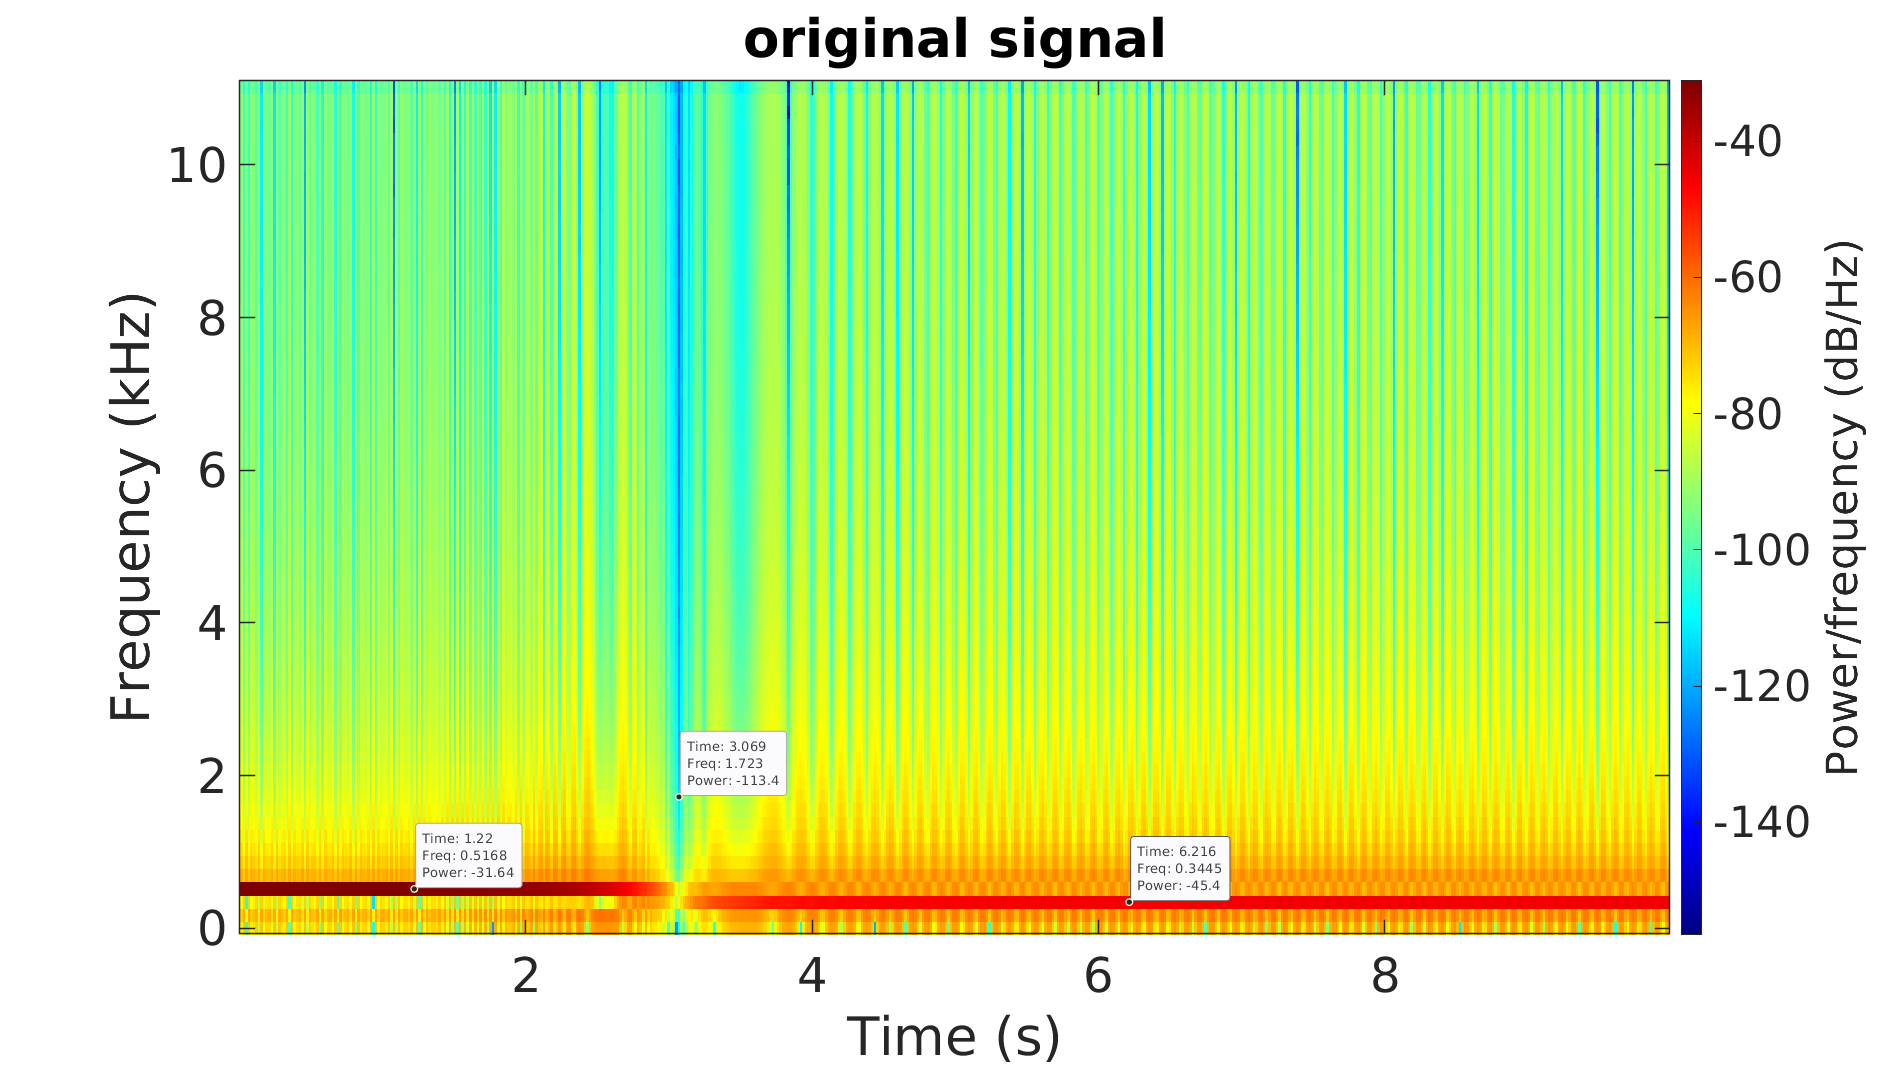
\includegraphics[width=0.9\textwidth]{figs/ex1_spectrogram_orig.png}
	\caption{Spectrogram of the given signal.}
	\label{fig:spectrogram_original}
\end{figure}

This, approach lead to $xObs = 56.8$ and $dObs = 10$.




% \section{Problem 2}

\subsection{Instruction}

Show that the group velocity vg and the phase index of refraction np are related
by $v_g = c \eta_p$ for small group and phase velocity departures from the speed
of light $c$.

\subsection{Solution}



\section{Problem 3}

\subsection{Instruction}

In lecture we considered an analog signal $x_a (t)$ sampled by impulses:

\begin{equation}
	x_\delta (t) = \sum_{n=-\infty}^{\infty} x_a(nT) \delta(t-nT)
	\label{eq:ex3_analog_signal}
\end{equation}

We showed that the Fourier transform of the impulse-sampled signal $x_\delta (t)$
is related to $X_a (f)$, the Fourier transform of $x_a (t)$, by

\begin{equation}
	X_\delta (f) = \frac{1}{T} \sum_{n=-\infty}^{\infty} X_a(f- \frac{n}{T})
	\label{eq:ex3_FT_sampled_signal}
\end{equation}

We can derive a similar relationship between $X_a (f)$ and the Fourier transform
of the discrete-time signal

\begin{equation}
	x(n) = x_a (nT), − \infty < n < \infty
\end{equation}

To make this easier, we’ll define the frequency variable
$\tilde{f} = f T = \frac{f}{f_s}$. This variable, which has units of cycles per
sample and is often called the normalized frequency, is used as the frequency
variable for discrete-time signals. For example, a discrete-time sinusoid can be
represented as $2x(n) = cos(2\pi \tilde{f}n)$. For discrete-time signals, only
frequencies in the range $− 1/2 \le \tilde{f} \le 1/2$ are unique;
all frequencies $|\tilde{f}| > 1/2$ are aliases.

The Fourier transform of a discrete-time signal $x(n)$ is defined by

\begin{equation}
	X(\tilde{f}) = \sum_{n=-\infty}^{\infty} x(n) \exp{(-j 2 \pi \tilde{f} n)}
	\label{eq:ex3_DFT}
\end{equation}

and the inverse transform is defined by

\begin{equation}
	x(n) = \int_{-1/2}^{1/2} X(\tilde{f}) \exp{(j 2 \pi \tilde{f} n)} d\tilde{f}
	\label{eq:ex3_IDFT}
\end{equation}

Derive the relationship between $X(\tilde{f})$ and $X_a (f)$.

\textbf{Hint:} This is a standard relationship whose derivation can be found in
many texts that treat digital signal processing. You’re free to use such a text
as a guide or you may perform the derivation yourself following these steps:

\begin{itemize}
	\item Express $x(n) = x_a (nT)$ in terms of $X_a (f)$.
	\item Equate this expression with the inverse transform definition given above.
	\item Express the integral that goes from $−\infty to \infty$ as an infinite
	      sum of integrals of width $f_s$.
	\item Make a change of variable $f = \tilde{f}  fs$ in this infinite sum of
	      integrals expression to eliminate $f$ in favor of $\tilde{f}$.
	\item Make some deductions to arrive at the desired relationship between
	      $X(\tilde{f})$ and $X_a (f = \tilde{f}·fs )$.
\end{itemize}

\subsection{Solution}

It is possible to consider equation~\ref{eq:ex3_analog_signal} to calculate the
Fourier Transform of $x_\delta(t)$.

\begin{equation}
	X_\delta (f) = \frac{1}{T} \sum_{n=-\infty}^{\infty} X_a(f- \frac{n}{T})
	= \sum_{n=-\infty}^{\infty} x_a(nT) \exp{(-j 2 \pi f n T)}
\end{equation}

Then, it is possible to see that formula for $X_\delta (f)$ can be equated to
\ref{eq:ex3_DFT} as follows

\begin{equation}
	X_\delta (f) = \sum_{n=-\infty}^{\infty} x_a(nT) \exp{(-j 2 \pi f n T)}
	= \sum_{n=-\infty}^{\infty} x(n) \exp{(-j 2 \pi \tilde{f} n)}
	= X(\tilde{f})
\end{equation}

This leads to the following relationship

\begin{equation}
	X(\tilde{f}) = X_\delta (\frac{\tilde{f}}{T})
\end{equation}

Now, using equation~\ref{eq:ex3_FT_sampled_signal} it is possible to reach

\begin{equation}
	X(\tilde{f}) = \frac{1}{T} \sum_{n=-\infty}^{\infty} X_a(\frac{\tilde{f}- n}{T})
\end{equation}

% \section{Problem 4}

\subsection{Instruction}

To measure the receiver temperature $T_R$ of a GNSS receiver and antenna setup,
a friend recommends placing the receiver’s antenna in a RF test enclosure such
as the one in the Radionavigation Laboratory (seen here
https://ramseytest.com/forensic-test-enclosures),
but cryogenically cooled down to 5 K, and then measuring the noise power in the
raw samples generated by the receiver. The enclosure effectively isolates the
antenna from environmental noise. The antenna is an active antenna consisting of
a patch element, a (passive) filter, and an amplifier. Is this a valid approach
for measuring TR ? Why or why not?

\subsection{Result}

The cryogenically cooled enclosure would only allow us to reduce the noise of
the receiver but not $T_A$. Therefore one could measure the noise power with and
without the cryogenically cooled enclosure and get an estimate of the $T_R$ by
substracting the results.

It seems like this is not a good idea though because if one would like to make the
best use of their money for the general usage of the GNSS receiver. Then, buying
the cryogenically cooled enclosure would only buy you a couple dBs better noise
performance. The main source of noise (the other GNSS signals one is not
interested in when aquiring from a particular satellite) would not be attenuated.
Therefore, one could measure the desired magnitude but that's it. No noticible
benefit would come from this purchase.



\section{Problem 5}

\subsection{Instruction}

Write a function in Matlab for computing the ionospheric delay from a model of
the ionosphere. Your function should adhere to the interface described on the
next page (which you can copy and paste as comments to your function). Only
develop calculations for the broadcast (Klobuchar) model. The function can later
be augmented to accommodate other model types. You can learn about the broadcast
model on pages 168-169 of the Misra and Enge text. More details can be found on
pages 128-130 of the GPS interface specification (IS) IS-GPS-200F.pdf posted on
Canvas. You will also need to write your own function for computing satellite
elevation and azimuth angles. Assume the WGS84 model for the shape of the Earth.
Note that the GPS IS uses semicircles as its angular measure, which is a strange
convention employed back in the 1970s to reduce memory and computation
requirement. The sin and cos functions in the IS (e.g., in Fig. 20-4) are meant
to operate on semicircles, unless otherwise indicated. Thus, when the IS writes,
e.g., $cos(\lambda_i −1.1617)$, where $\lambda_i$ is given in semicircles, you
can implement this in Matlab as $cos((\lambda_i −1.1617)\pi)$.

\subsection{Solution}


\begin{lstlisting}
function [delTauG] = getIonoDelay(ionodata,fc,rRx,rSv,tGPS,model)
% getIonoDelay : Return a model-based estimate of the ionospheric delay
%                experienced by a trans-ionospheric GNSS signal as it
%                propagates from a GNSS SV to the antenna of a terrestrial
%                GNSS receiver.
%
% INPUTS
%
% ionodata ------- Structure containing a parameterization of the
%                  ionosphere that is valid at time tGPS. The structure is
%                  defined differently depending on what ionospheric model
%                  is selected:
%
%                  broadcast --- For the broadcast (Klobuchar) model, ionodata
%                                is a structure containing the following fields:
%
%                       alpha0 ... alpha3 -- power series expansion coefficients
%                                            for amplitude of ionospheric delay
%                       beta0 ... beta3 -- power series expansion coefficients
%                                          for period of ionospheric plasma density 
%                                          cycle
%
%
% Other models TBD ...
%
% fc ------------- Carrier frequency of the GNSS signal, in Hz.
%
% rRx ------------ A 3-by-1 vector representing the receiver antenna position
%                  at the time of receipt of the signal, expressed in meters
%                  in the ECEF reference frame.
%
% rSv ------------ A 3-by-1 vector representing the space vehicle antenna
%                  position at the time of transmission of the signal,
%                  expressed in meters in the ECEF reference frame.
%
% tGPS ----------- A structure containing the true GPS time of receipt of
%                  the signal. The structure has the following fields:
%                  week -- unambiguous GPS week number
%                  seconds -- seconds (including fractional seconds) of the
%                  GPS week
%
% model ---------- A string identifying the model to be used in the
%                  computation of the ionospheric delay:
%                  broadcast --- The broadcast (Klobuchar) model.
%
% Other models TBD ...
%
% OUTPUTS
%
% delTauG -------- Modeled scalar excess group ionospheric delay experienced
%                  by the transionospheric GNSS signal, in seconds.
%
%+----------------------------------------------------------------------------+
% References: For the broadcast (Klobuchar) model, see IS-GPS-200F
% pp. 128-130.
%
%+============================================================================+
wgs84 = wgs84Ellipsoid('meter');
[lat,lon,h] = ecef2geodetic(wgs84, rRx(1), rRx(2), rRx(3));
[az,elev,slantRange] = ecef2aer(rSv(1), rSv(2), rSv(3), lat, lon, h, wgs84);
lambda_u = lon/180; % user geodetic longitude (semi-circles)
phi_u    = lat/180; % user geodetic latitude (semi-circles) 
A        = az/180;  % azimuth angle between user and satellite, measured clockwise 
                % positive from the true North (semi-circles) 
E        = elev/180;% elevation angle between user and satellite (semi_circle)

% earth's  central  angle  between  the  user  position  and  the  earth  
% projection  of ionospheric intersection point (semi-circles) 
Psi = 0.0137/(E+0.11) - 0.022;

% geodetic  latitude  of  the  earth  projection  of  the  ionospheric  
% intersection  point (semi-circles) 
phi_i = phi_u + Psi * cos(A*pi);
phi_i = max(-0.416, phi_i);
phi_i = min(0.416, phi_i);

% geodetic  longitude  of  the  earth  projection  of  the  ionospheric  
% intersection  point (semi-circles) 
lambda_i = lambda_u + Psi*cos(A*pi)/cos(phi_i*pi);

% geomagnetic latitude of the earth projection of the ionospheric 
% intersection point (mean ionospheric height assumed 350 km) (semi-circles) 
phi_m = phi_i + 0.064*cos((lambda_i - 1.617)*pi);

% local time (sec) 
t = 4.32*(10^4)*lambda_i + tGPS.seconds;
while t > 86400
    t = t - 86400;
end
while t < 0
    t = t + 86400;
end

PER = ionodata.broadcast.beta0 * phi_m^0 + ...
      ionodata.broadcast.beta1 * phi_m^1 + ...
      ionodata.broadcast.beta2 * phi_m^2 + ...
      ionodata.broadcast.beta3 * phi_m^3;
PER = max(72000, PER);


AMP = ionodata.broadcast.alpha0 * phi_m^0 + ...
      ionodata.broadcast.alpha1 * phi_m^1 + ...
      ionodata.broadcast.alpha2 * phi_m^2 + ...
      ionodata.broadcast.alpha3 * phi_m^3;
AMP = max(0, AMP);

% phase (radians) 
x = 2*pi*(t - 50400)/PER;

% obliquity factor (dimensionless) 
F = 1 + 16*(0.53 - E)^3;

% Estimate the ionospheric delay
if abs(x) < 1.57
    T_iono = F*(5e-9 + AMP * (1 - (x^2)/2 + (x^4)/24));
else
    T_iono = F * 5e-9;
end

if fc == 1227.44 * 1e6
    gamma = (77/60)^2;
    T_iono = gamma * T_iono;
end

delTauG = T_iono;
end
\end{lstlisting}

\subsection{Results}

The solution I got for the conditions provided was $delTauG = 23.3269 ns$, which
translates to about 7 meters.

% \section{Problem 6}

\subsection{Instruction}

If C(t) is a random binary (± 1) spreading code with rectangular pulses, then,
as we showed in lecture, the power spectral density of C(t) is given by

\begin{equation}
	S_C (f) = T_C sinc^2 (f T_C )
\end{equation}

where $T_C$ is the chipping interval.

Suppose instead that C(t) has psd

\begin{equation}
	S_C (f) = T_C \Pi(f T_C )
\end{equation}

where $\Pi(f)$ is the rect function introduced in lecture. Imagine a
constellation of GNSS satellites broadcasting signals having this new $S_C (f)$.
Assume the signals have no data bit modulation, so that the signal’s baseband
representation is of the form

\begin{equation}
	r(t) = \sqrt{P} C(t) \exp[j \theta(t)]
\end{equation}

For this case, calculate $I_0 = S_I(0)$ for a single multiple-access interference
signal with power $P_I$, where $I_0$ and $S_I (f)$, the power spectrum of $I(t)$,
were defined in lecture. Now consider M multiple-access signals (including the
desired signal). If each of the M received signals has power $P_I$, at what value
of M does $I_0$ exceed $N_0$ ? Express your answer in terms of $N_0$, $T_C$ and
$P_I$.

\subsection{MATLAB code}

\begin{lstlisting}
%% Problem 4
% Suppose that C(t) has a power spectral density given by:
%
%                   Sc(f) = Tc * rectangularPulse(f*Tc)
%
% Where 'rectangularPulse' is the rect function introduced in lecture.
% Imagine a constellation of GNSS satellites broadcasting signals having
% this new Sc(f). Assume the signals have no data bit modulation, so that
% the signal's baseband representation is of the form:
%
%                   r(t) = sqrt(P)*C(t)*exp[j theta(t)]
%
clc, close all, clear all

% For this case, calculate I0 = SI(f=0) for a single multiple-access
% interference signal with power PI, where I0 and SI(f), the power spectrum
% of I(t), were defined in class.
%
% ANSWER:
% Following the same reasoning as in lecture:
% If CI(t) is a random-binary sequence "like C(t)" (same Tc), and if the
% two are uncorrelated. Then, (assuming fD=0)
%                       
%                   SrI(f) = PI*Sc(f)
% Thus, 
%                   SI(f) = Sc(f) x SrI(f) = Sc(f) x (PI*Sc(f))
%
%                   SI(f) = PI * integral_{-inf}^{inf}(Sc(f-x)Sc(x) dx
%
% Since, Sc(f) = Sc(-f)
%
%                   SI(f) = PI * integral_{-inf}^{inf}(Sc(x-f)Sc(x) dx
%
% Now, using the fact that the receiver has a low pass filter, only the f=0
% part of the spectral density leaks through. Therefore, it's ok to assume 
% I0 = SI(f=0) (REMEMBER: I0 is also a power density)
%
%     SI(0) = PI * integral_{-inf}^{inf}(Sc(x)^2) dx
%
%     SI(0) = PI * integral_{-inf}^{inf}(Tc*rectangularPulse(x*Tc)^2) dx
%
%     SI(0) = PI*Tc
I0 = PI*Tc;
I0_dBW_Hz = 10*log10(I0)

% Now consider M multiple-access signals (including the desired signal). If
% each of the M received signals has power PI, at what value of M does I0
% exceed N0? Express your answer in terms of N0, Tc, PI.
%
% ANSWER:
% The multiple-access interference is characterized by:
%
%           I0 = PI*Tc*(M-1)
%
% We want to know what M would result in I0 >= N0
%
%           PI*Tc*(M-1) >= N0
%           M >= N0/(PI*Tc) + 1, where M is integer
%        
% => I0 exceeds N0 when:
%           M = ceil(N0/(PI*Tc) + 1)
%
\end{lstlisting}

% \section{Problem 7}

In this problem we’ll further analyze the data taken with the Stanford 46-meter
diameter dish. The gain of the Stanford dish is so great (about 50 dB at the GPS
L1 frequency) that you can actually see the transitions induced by the GPS L1
C/A code and by the GPS L1 P(Y) code. Recall that in lecture the GPS L1 signal
structure was presented as

\begin{equation}
	S_{L1} (t) = \sqrt{2P_{C1}} D(t) C(t) cos(2 \pi f_{L1} t + \theta_{L1} ) +
	\sqrt{2P_{Y1}} D(t) Y(t) sin(2 \pi f_{L1} t + \theta_{L1} )
\end{equation}

You can see from this that the GPS C/A code (spreading code C(t), chipping at
1.023 MHz) is in phase quadrature with the GPS Y code (spreading code Y (t),
chipping at 10.23 MHz).

Load the “Big Dish” data into your workspace in Matlab (you can use the
bigDishPSD.m script to do this). The sampling rate for these data is
$fs = 46.08 MHz$. The data are loaded into the Matlab complex variable Y. Each
element in Y represents a complex sample of the GPS signal $S_{L1}(t)$ after
mixing to baseband. The researchers who recorded the data mixed the incoming
signal to baseband with a fairly accurate estimate of the signal’s instantaneous
center frequency (including Doppler). Hence, the baseband samples have only a
small residual frequency, which gives rise to a slow rotation in the phase. If
you only look at, say, 400 samples, the phase doesn’t change much and you can
see a pattern emerge when you plot individual samples in the complex plane. (If
you look at much more than 400 samples, the slow phase rotation turns this
pattern into a donut shape.) Generate a plot similar to Fig. 1 by finding a
window of 400 samples of data within Y whose real and imaginary components form
a square that is aligned with the plot axes. Having identified such a window,
look at the real and imaginary components of Y over this window in the time
domain. Identify for your plot what signal component from SL1 (t) happens to be
in real(Y) and what component happens to be in imag(Y) over this window. Measure
the smallest chip interval for both codes. Estimate from your data the ratio of
the C/A code amplitude to the P (Y ) code amplitude.

\subsection{MATLAB code}

\begin{lstlisting}
%% Problem 6
clear all; clc; close all;
addpath("research/toolbox/")

%----- Load data
load('prn31_22apr03_01hrs40min00sec_gmt_fl1_46_08mhz_250msec.mat');

start = 8000;
Y_windowed = Y(start:start+400,:);

% Plotting the complex representation of the signal such that it forms a
% "perfect" square in the the complex plane.
figure()
plot(Y_windowed,'.')
xlabel('In phase');
ylabel('Quadrature');
title('Complex representation of the baseband signal');

t = XDelta*(0:400) * 1e6;
CA_code = real(Y_windowed);
Y_code = imag(Y_windowed);

% Plotting the real and imaginary parts of the signal
figure()
subplot(2,1,1)
    plot(t,CA_code)
    xlabel('time [us]');
    ylabel('X_{In-phase}');
    title('Time-domain representation of X_{In-phase}');

subplot(2,1,2)
    plot(t, Y_code)
    xlabel('time [us]');
    ylabel('X_{Quadrature}');
    title('Time-domain representation of X_{Quadrature}');

% The ratio of the C/A code amplitude to the P(Y) code amplitude
ratio = mean(sqrt(CA_code.^2)) / mean(sqrt(Y_code.^2)) % Amplitude of C/A_code is ~1.4x P(Y) code amplitude 
\end{lstlisting}

\subsection{Results}

Figure~\ref{fig:ex7_quadrature} shows the complex representation of the signals
in phase-quadrature.

\begin{figure}[H]
	\centering
	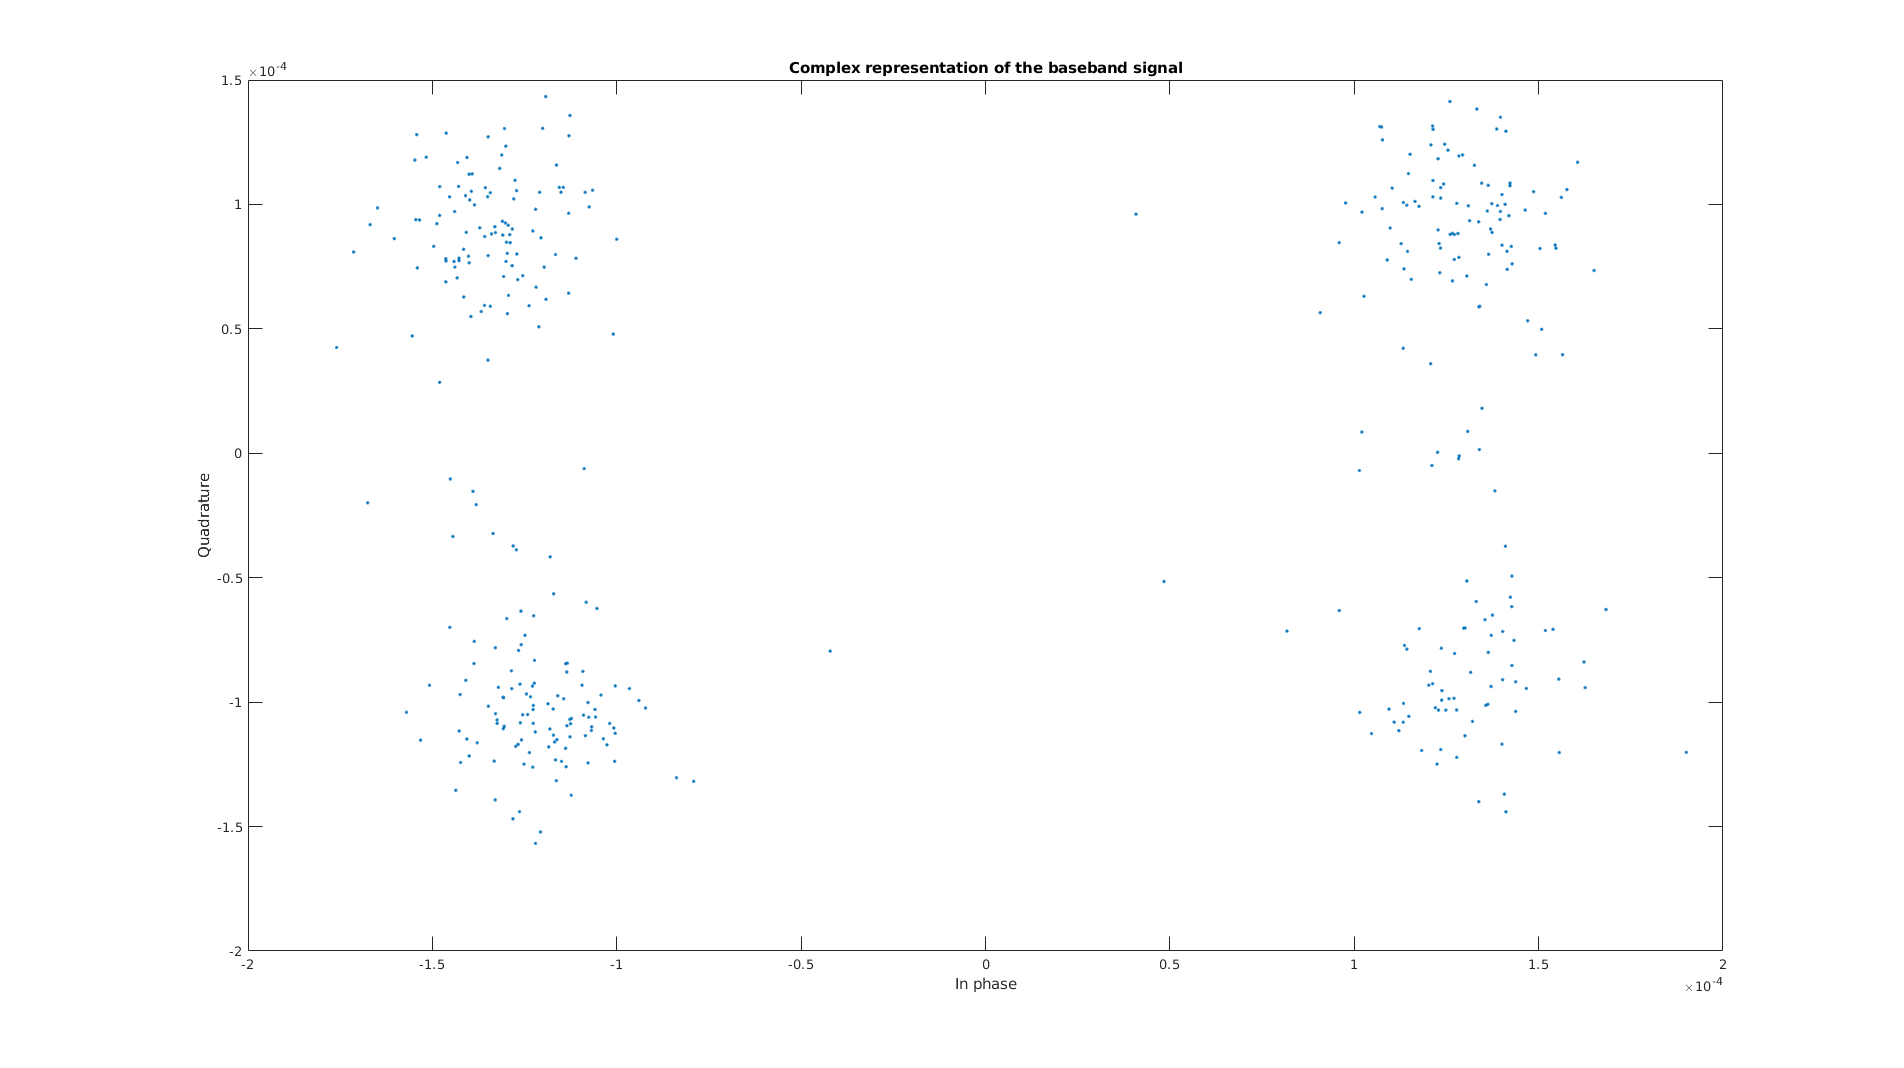
\includegraphics[width=0.9\textwidth]{figs/ex7_quadrature.png}
	\caption{Individual samples of the Stanford "Big Dish" data plotted in the
		complex plane.}
	\label{fig:ex7_quadrature}
\end{figure}

Figure~\ref{fig:ex7_time_domain}, shows the time-domain representation of the
previously shown phase-quadrature signals. It it possible to distinguish the
GPS L1 C/A-code in the top plot. It can be appreciated from the graph that the
period of the signal is $~1 \mu s$. The bottom graph exposes the P(Y)-code,
characterized by its faster chipping of $~0.1 \mu s$.

\begin{figure}[H]
	\centering
	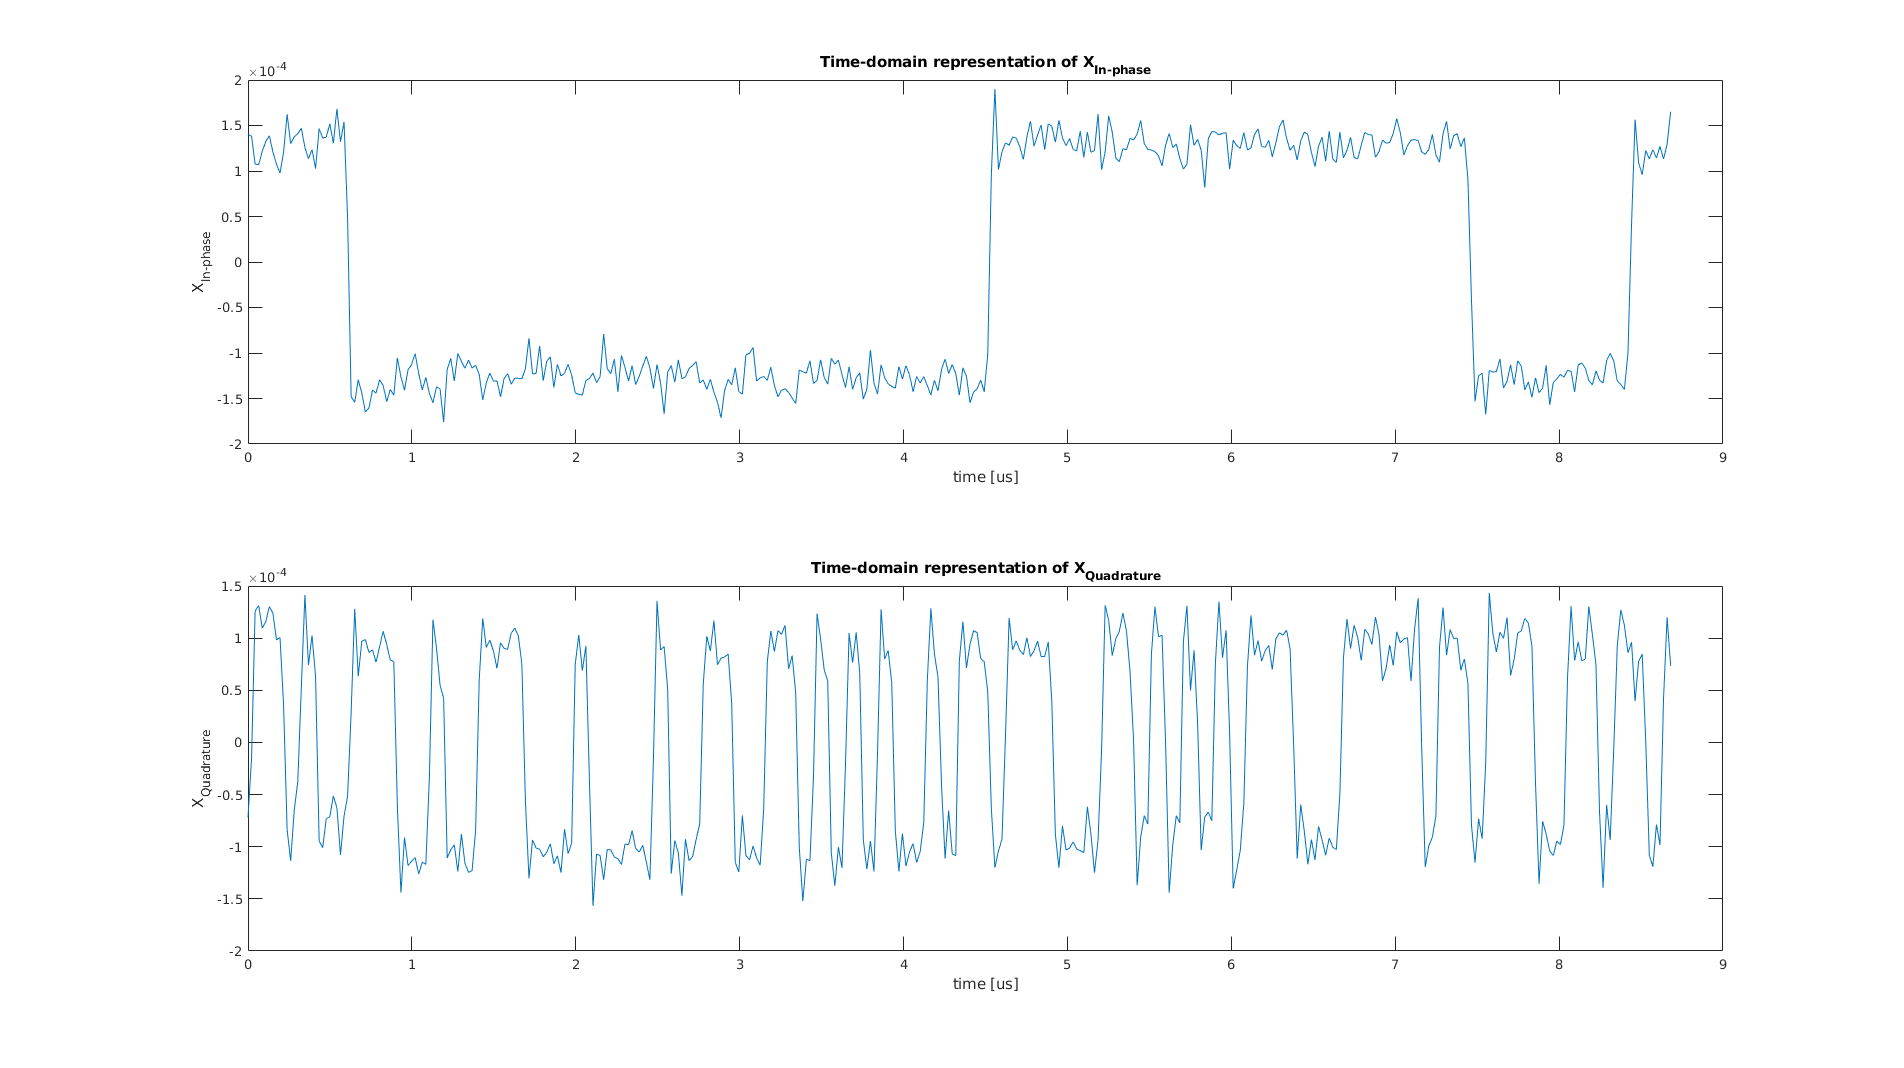
\includegraphics[width=0.9\textwidth]{figs/ex7_time_domain.png}
	\caption{Time-domain representation of the signals previously shown in
		phase-quadrature.}
	\label{fig:ex7_time_domain}
\end{figure}

Finally, the ratio of the C/A-code amplitude to the P(Y)-code amplitude reveals
that the C/A-code amplitude is $~1.4$ times larger than P(Y)-code amplitude.


% \section{Problem 8}

\subsection{MATLAB code}

\begin{lstlisting}
%% Problem 9a

% correlationExperiments.m
%
% Experiment with properties of pseudorandom sequences.


clear;clc;
addpath("research/toolbox/")
%----- Setup
nStages = 10;                 % Number of stages in LFSR
Tc = 1e-3/1023;               % Chip interval in seconds
delChip = 3/217;              % Sampling interval in chips
delOffset  = 0;               % Offset of first sample
delt = delChip*Tc;            % Sampling interval in seconds
fs = 1/delt;                  % Sampling frequency in Hz
Np = 2^nStages - 1;           % Period of the sequence in chips
Nr = 20;                      % Number of repetitions of the sequence
Ns = round(Nr*Np/delChip);    % Number of samples of the sequence 

N = 10000;
varVec = zeros(N,1);
for i=1:N
    % codeType:
    % rand ---- Sequence derived from Matlab randn function
    % pi ------ Sequence derived from the digits of pi
    % mseq ---- Maximal-length sequence with n = nStages
    codeType = 'rand';
    
    %----- Generate codes
    X1 = zeros(Np,1);
    X2 = zeros(Np,1);
    if(strcmp(codeType,'rand'))
      X1 = sign(sign(randn(Np,1)) + 0.1);
      X2 = sign(sign(randn(Np,1)) + 0.1);
    elseif(strcmp(codeType,'pi'))
      [sPi,vPi] = pi2str(2*Np);
      X1 = vPi(1:Np) >= 5;
      X1 = 2*X1 - 1;
      X2 = vPi(Np+1:2*Np) >= 5;
      X2 = 2*X2 - 1;
    elseif(strcmp(codeType,'mseq'))
    ciVec1 = [9, 4]';  
    ciVec2 = [9, 2]';
    a0Vec1 = [1;zeros(nStages-1,1)];
    a0Vec2 = ones(nStages,1);
    X1 = generateLfsrSequence(nStages,ciVec1,a0Vec1);
    X2 = generateLfsrSequence(nStages,ciVec2,a0Vec2);
    X1 = 2*X1 - 1;
    X2 = 2*X2 - 1;
    else
      error('Unrecognized code type');
    end
    
    %----- Compute the sequence crosscorrelation
    [Rseq12,iiVecSeq] = ccorr(X1,X2);
    index = find(iiVecSeq==0);
    crosscorrVec(i) = Rseq12(index);
end

% The problem asks about the variance of the cross-correlation at k=0
var(crosscorrVec)
\end{lstlisting}

\begin{lstlisting}
%% Problem 9b

% correlationExperiments.m
%
% Experiment with properties of pseudorandom sequences.


clear;clc; format short
addpath("research/toolbox/")
%----- Setup
nStages = 10;                 % Number of stages in LFSR
Tc = 1e-3/1023;               % Chip interval in seconds
delChip = 3/217;              % Sampling interval in chips
delOffset  = 0;               % Offset of first sample
delt = delChip*Tc;            % Sampling interval in seconds
fs = 1/delt;                  % Sampling frequency in Hz
Np = 2^nStages - 1;           % Period of the sequence in chips
Nr = 20;                      % Number of repetitions of the sequence
Ns = round(Nr*Np/delChip);    % Number of samples of the sequence 

N = 6;
varVec = zeros(N,1);
for i=1:N
    ciVec1 = [
        [10, 9, 8, 5]',...  
        [10, 9, 7, 6]',...
        [10, 9, 7, 3]',...
        [10, 9, 6, 1]',...
        [10, 9, 5, 2]',...
        [10, 9, 4, 2]'
    ];
    ciVec2 = [
        [10, 9, 8, 7, 5, 4]',...  
        [10, 9, 8, 7, 4, 1]',...
        [10, 9, 8, 7, 3, 2]',...
        [10, 9, 8, 6, 5, 1]',...
        [10, 9, 8, 6, 4, 2]',...
        [10, 9, 8, 6, 4, 2]'  
    ];
    a0Vec1 = [1;zeros(nStages-1,1)];
    a0Vec2 = ones(nStages,1);
    X1 = generateLfsrSequence(nStages,ciVec1(:,i),a0Vec1);
    X2 = generateLfsrSequence(nStages,ciVec2(:,i),a0Vec2);
    X1 = 2*X1 - 1;
    X2 = 2*X2 - 1;
    %----- Compute the sequence crosscorrelation
    [Rseq12,iiVecSeq] = ccorr(X1,X2);
    
    bound_crosscorrVec(i) = max(Rseq12);

    %----- Compute the sequence autocorrelation
    [Rseq11,iiVecSeq] = ccorr(X1,X1);
    index = find(iiVecSeq==0);
    autocorrVec(i) = Rseq11(index);
end

% The value of the autocorr at k=0 ~ (N-1)
autocorrVec

% The bound of the cross-correlation >= sqrt(N)
bound_crosscorrVec
\end{lstlisting}

\begin{lstlisting}
%% Problem 9c

clear;clc;close all
addpath("research/toolbox/")
%----- Setup
nStages = 10;                 % Number of stages in LFSR
Tc = 1e-3/1023;               % Chip interval in seconds
delChip = 3/217;              % Sampling interval in chips
delOffset  = 0;               % Offset of first sample
delt = delChip*Tc;            % Sampling interval in seconds
fs = 1/delt;                  % Sampling frequency in Hz
Np = 2^nStages - 1;           % Period of the sequence in chips
Nr = 20;                      % Number of repetitions of the sequence
Ns = round(Nr*Np/delChip);    % Number of samples of the sequence 
% codeType:
% rand ---- Sequence derived from Matlab randn function
% pi ------ Sequence derived from the digits of pi
% mseq ---- Maximal-length sequence with n = nStages
codeType = 'pi'; % Change this variable to see the different results

%----- Generate codes
X1 = zeros(Np,1);
X2 = zeros(Np,1);
if(strcmp(codeType,'rand'))
  X1 = sign(sign(randn(Np,1)) + 0.1);
  X2 = sign(sign(randn(Np,1)) + 0.1);
elseif(strcmp(codeType,'pi'))
  [sPi,vPi] = pi2str(2*Np);
  X1 = vPi(1:Np) >= 5;
  X1 = 2*X1 - 1;
  X2 = vPi(Np+1:2*Np) >= 5;
  X2 = 2*X2 - 1;
elseif(strcmp(codeType,'mseq'))
ciVec1 = [9, 4]';  
ciVec2 = [9, 2]';
a0Vec1 = [1;zeros(nStages-1,1)];
a0Vec2 = ones(nStages,1);
X1 = generateLfsrSequence(nStages,ciVec1,a0Vec1);
X2 = generateLfsrSequence(nStages,ciVec2,a0Vec2);
X1 = 2*X1 - 1;
X2 = 2*X2 - 1;
else
  error('Unrecognized code type');
end

%----- Oversample code
X1os = oversampleSpreadingCode(X1,delChip,delOffset,Ns,Np);
X2os = oversampleSpreadingCode(X2,delChip,delOffset,Ns,Np);

%----- Compute autocorrelation 
[R1,iiVec] = ccorr(X1os,X1os);
[R2,iiVec] = ccorr(X2os,X2os);

%----- Compute crosscorrelation 
[R12,iiVec] = ccorr(X1os,X2os);

ratio = max(R1)/max(R12)

%----- Compute power spectra
% The scaling here ensures that sum(Si*delf) = 1 W, as expected, for i = 1, 2.
S1 = abs(delt*fft(X1os)).^2/(Ns*delt);
S2 = abs(delt*fft(X2os)).^2/(Ns*delt);
S12 = abs(delt*fft(R12)).^2/(Ns*delt);
delf = 1/(delt*Ns);
fVec = [0:Ns-1]'*(delf);

%----- Scale for 1-Hz delf for plotting
% We'll present the power spectra in units of dBW/Hz, so we need to scale
% the spectra so that they match a delf = 1 Hz frequency spacing.
S1 = S1*delf;
S2 = S2*delf;
S12 = S12*delf;

%----- Plot
figure(1);clf;
subplot(211)
plot(iiVec,R1/Ns);
grid on;
ylabel('R_{X1}');
title('X1 and X2 autocorrelation')
subplot(212)
plot(iiVec,R2/Ns);
grid on;
ylabel('R_{X2}');
xlabel('Lag (samples)');
figure(2);clf;
plot(iiVec,R12/Ns);
title('X1 and X2 crosscorrelation')
xlabel('Lag (samples)');
grid on;
ylabel('R_{X1,X2}');
figure(3);clf;
subplot(211)
plot(fVec/1e3,10*log10(S1));
grid on;
xlim([0 30]);
ylim([-100,0]);
title('X1 and X2 power spectral densities')
ylabel('S_{X1}(f) (dBW/Hz)');
subplot(212)
plot(fVec/1e3,10*log10(S2));
grid on;
xlim([0 30]);
ylim([-100,0]);
ylabel('S_{X2}(f) (dBW/Hz)');
xlabel('Frequency (kHz)');
\end{lstlisting}


\subsection{Results}

\subsubsection{Item a}

The result verifies the claim

\subsubsection{Item b}

The result verifies the claim

\subsubsection{Item c}

\begin{figure}[H]
	\centering
	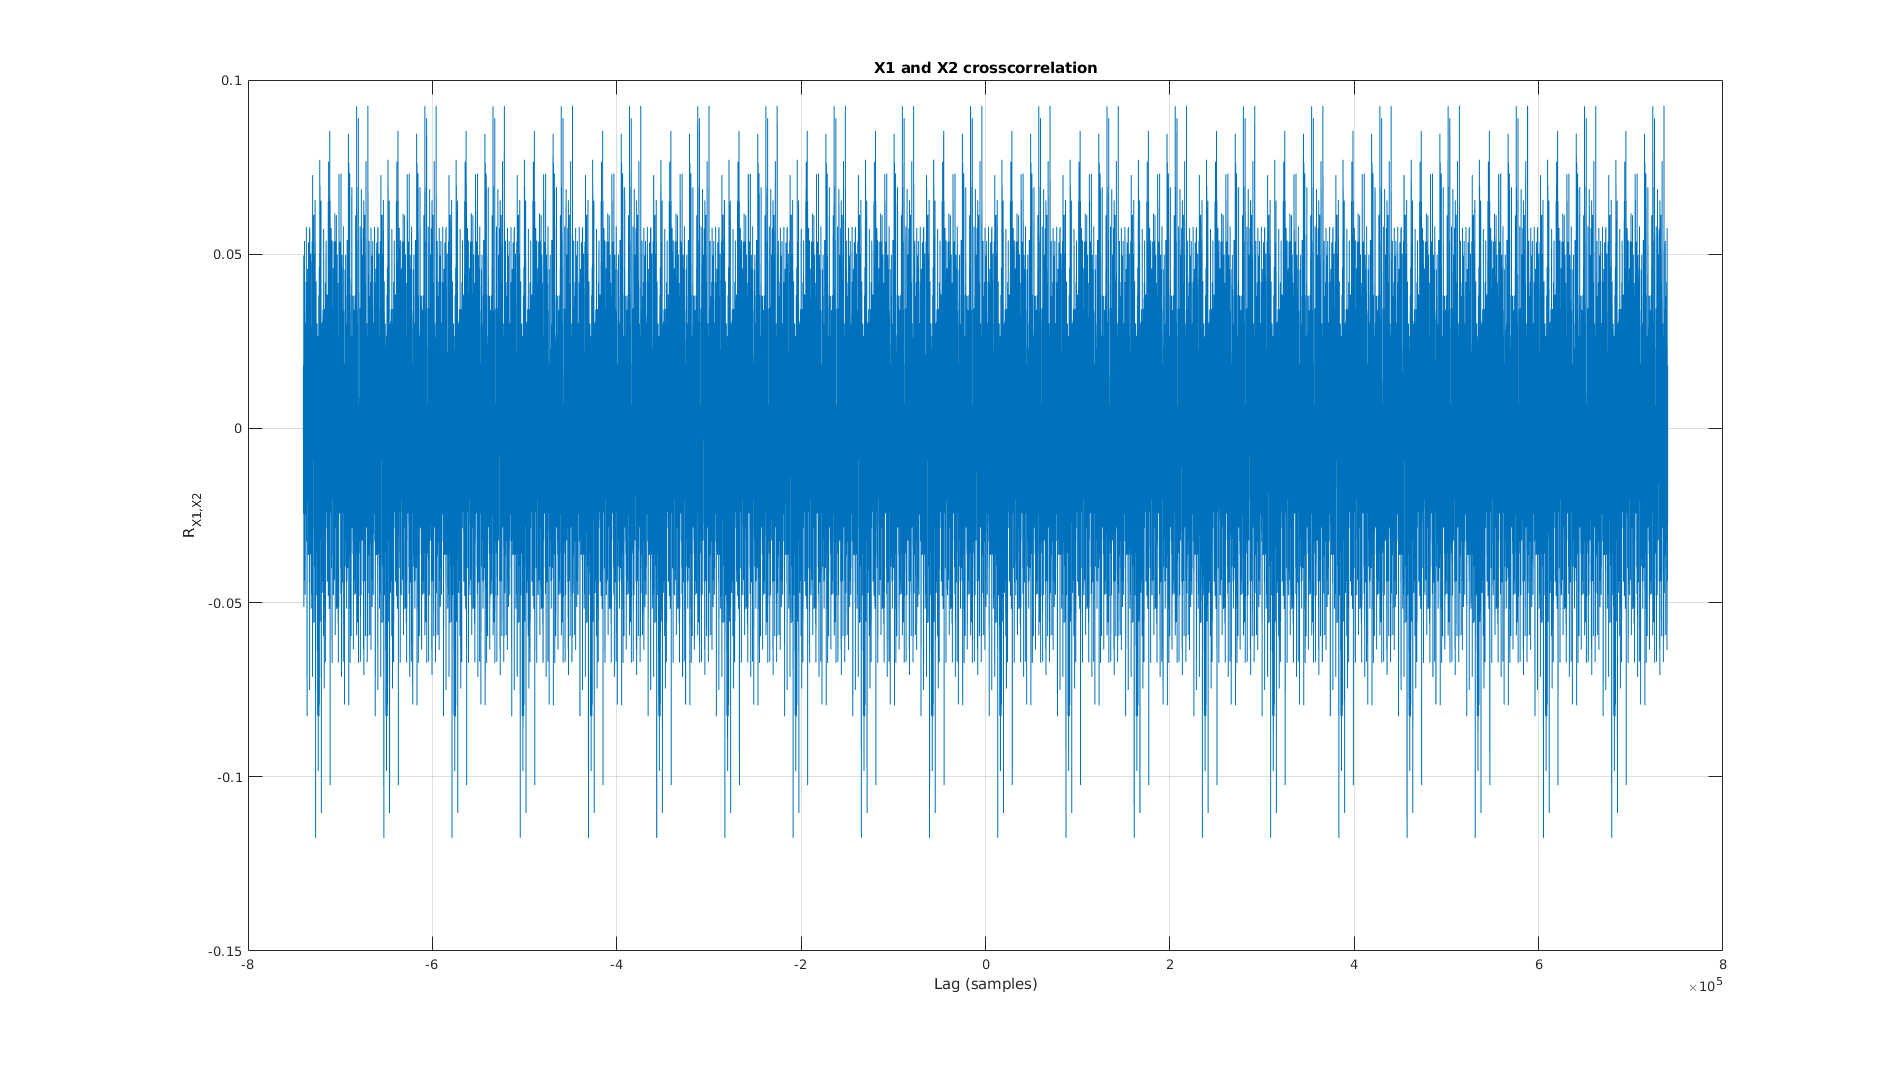
\includegraphics[width=0.9\textwidth]{figs/ex8_crosscorr_rand.png}
	\caption{Crosscorrelation of X1 and X2 for the \'rand\' case.}
	\label{fig:ex8_crosscorr_rand}
\end{figure}

\begin{figure}[H]
	\centering
	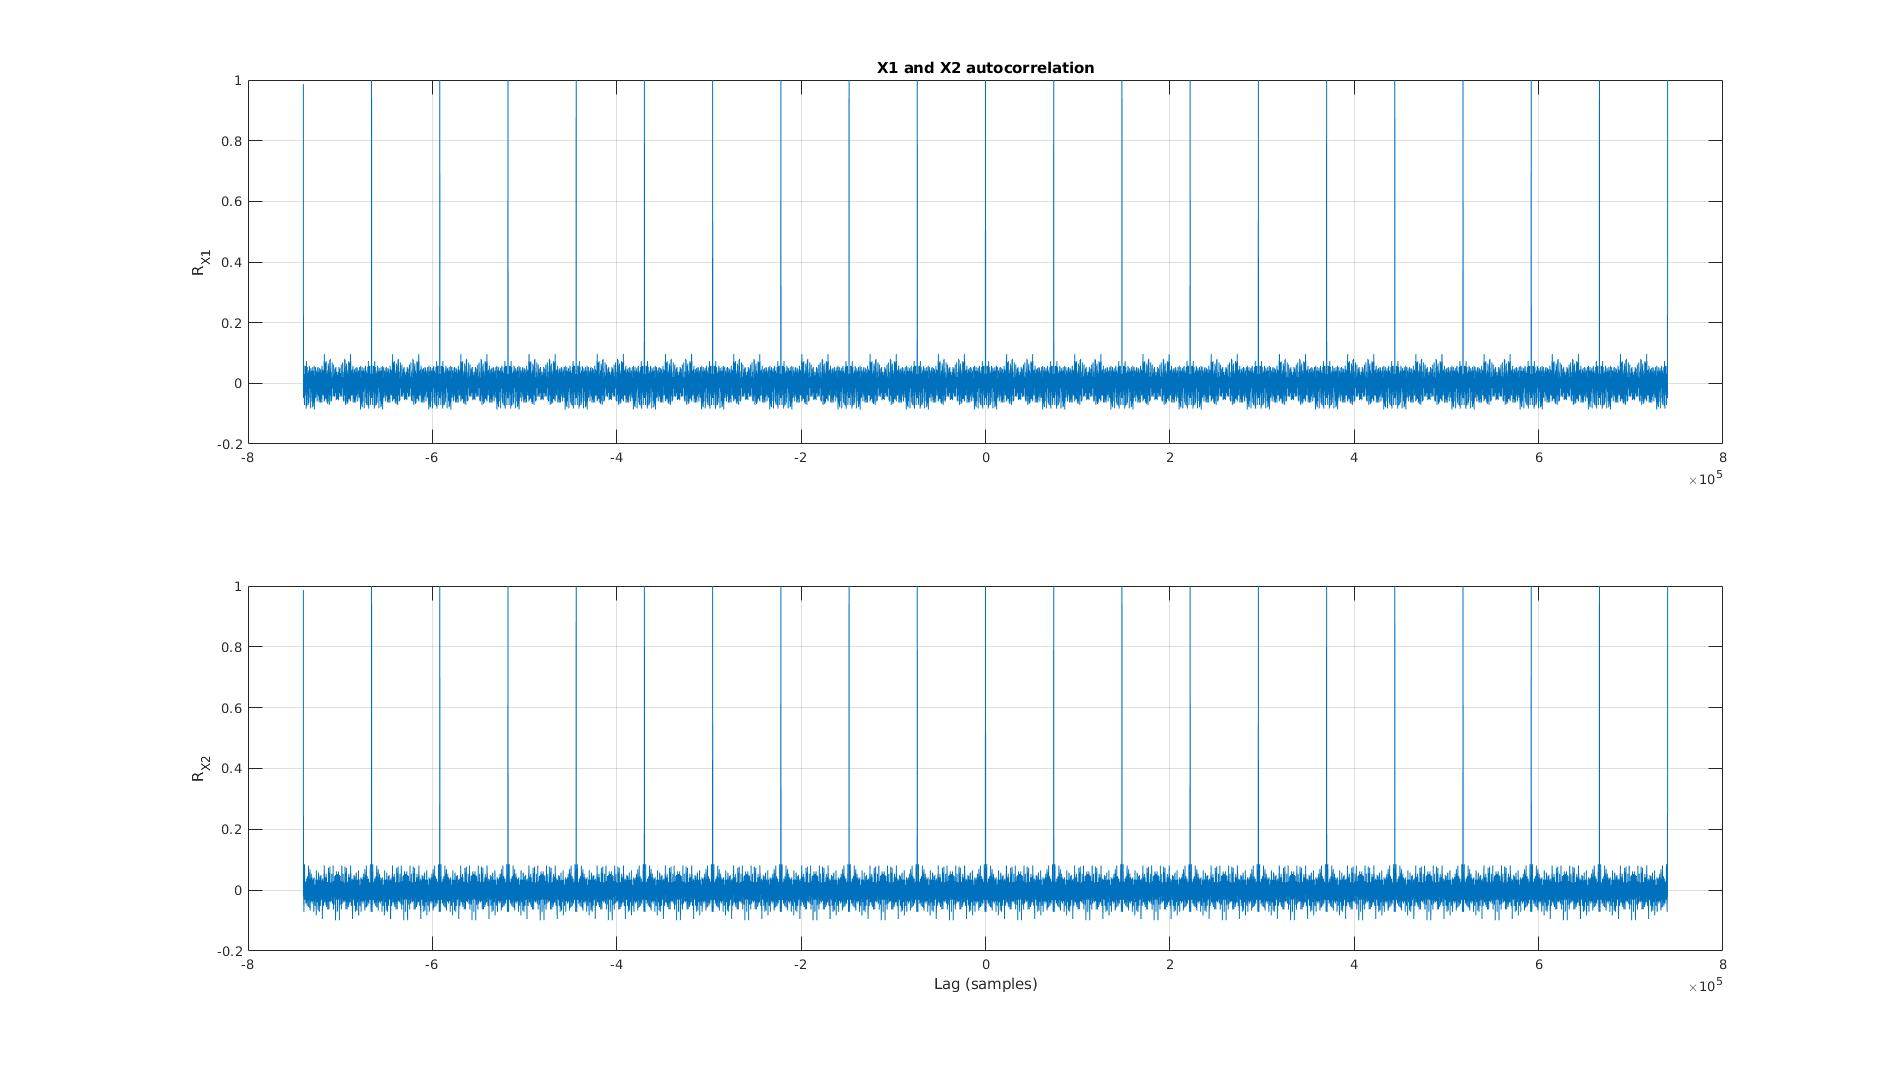
\includegraphics[width=0.9\textwidth]{figs/ex8_autocorr_rand.png}
	\caption{Autocorrelation of X1 and X2 for the 'rand' case.}
	\label{fig:ex8_autocorr_rand}
\end{figure}

\begin{figure}[H]
	\centering
	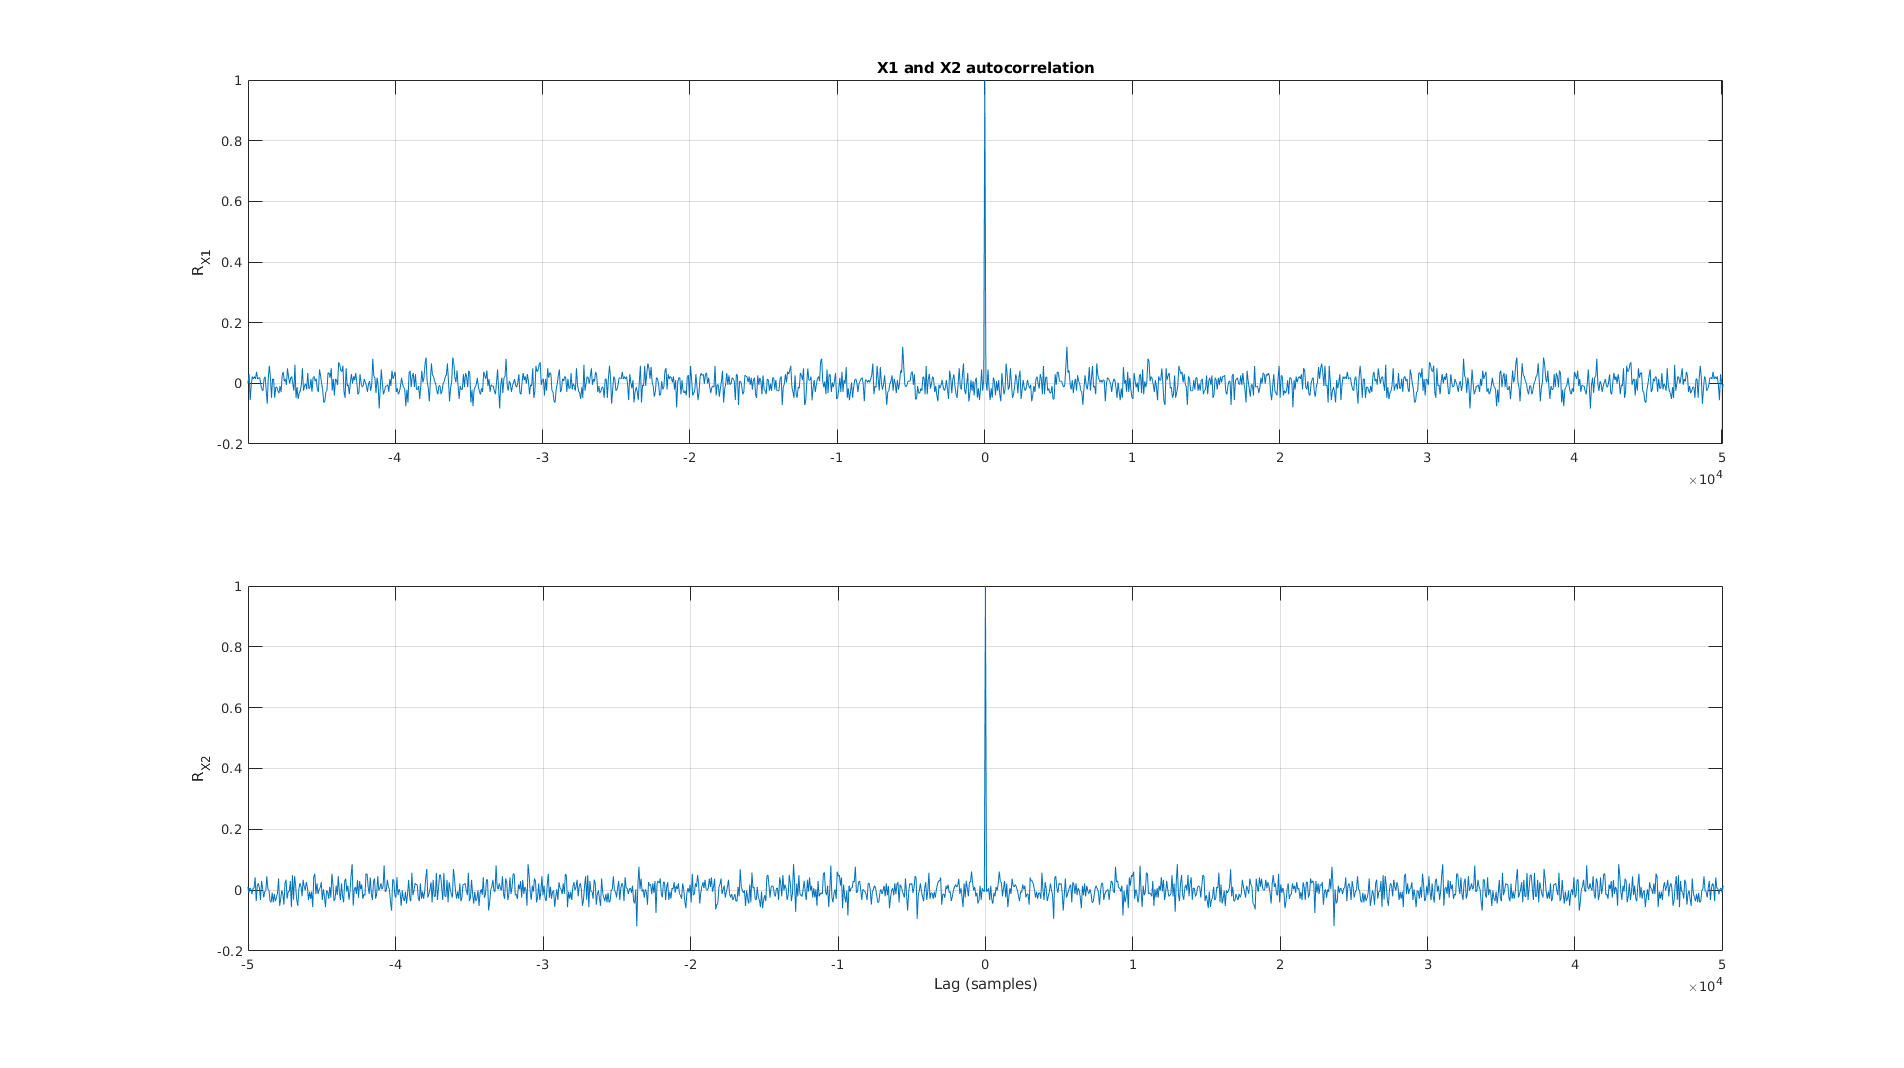
\includegraphics[width=0.9\textwidth]{figs/ex8_autocorr_zoomed_rand.png}
	\caption{Zoomed autocorrelation of X1 and X2 for the 'rand' case.}
	\label{fig:ex8_autocorr_zoomed_rand}
\end{figure}

The ratio of the maximum of $R_X(\tau)$ to the maximum of $R_{X1,X2}(\tau)$ is
11.54 for the case where we work with 'rand' method.

\begin{figure}[H]
	\centering
	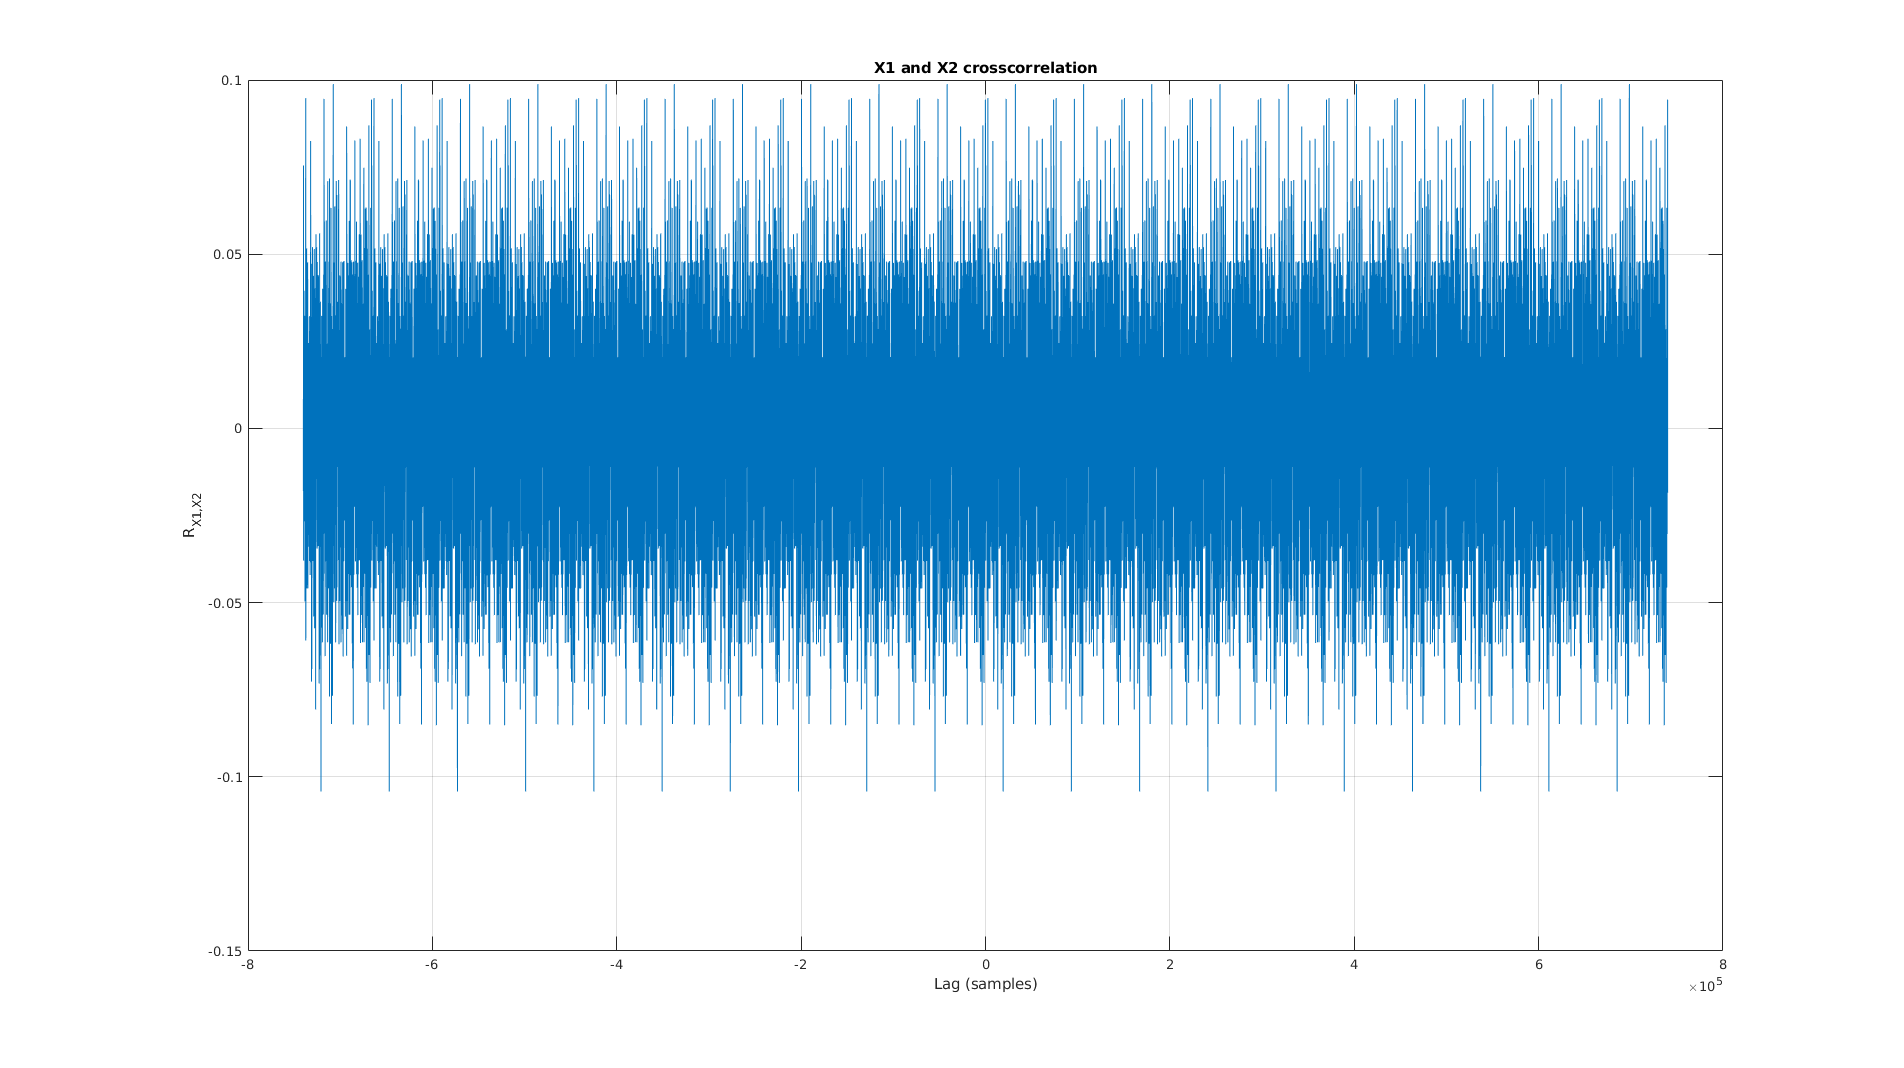
\includegraphics[width=0.9\textwidth]{figs/ex8_crosscorr_pi.png}
	\caption{Crosscorrelation of X1 and X2 for the 'pi' case.}
	\label{fig:ex8_crosscorr_pi}
\end{figure}

\begin{figure}[H]
	\centering
	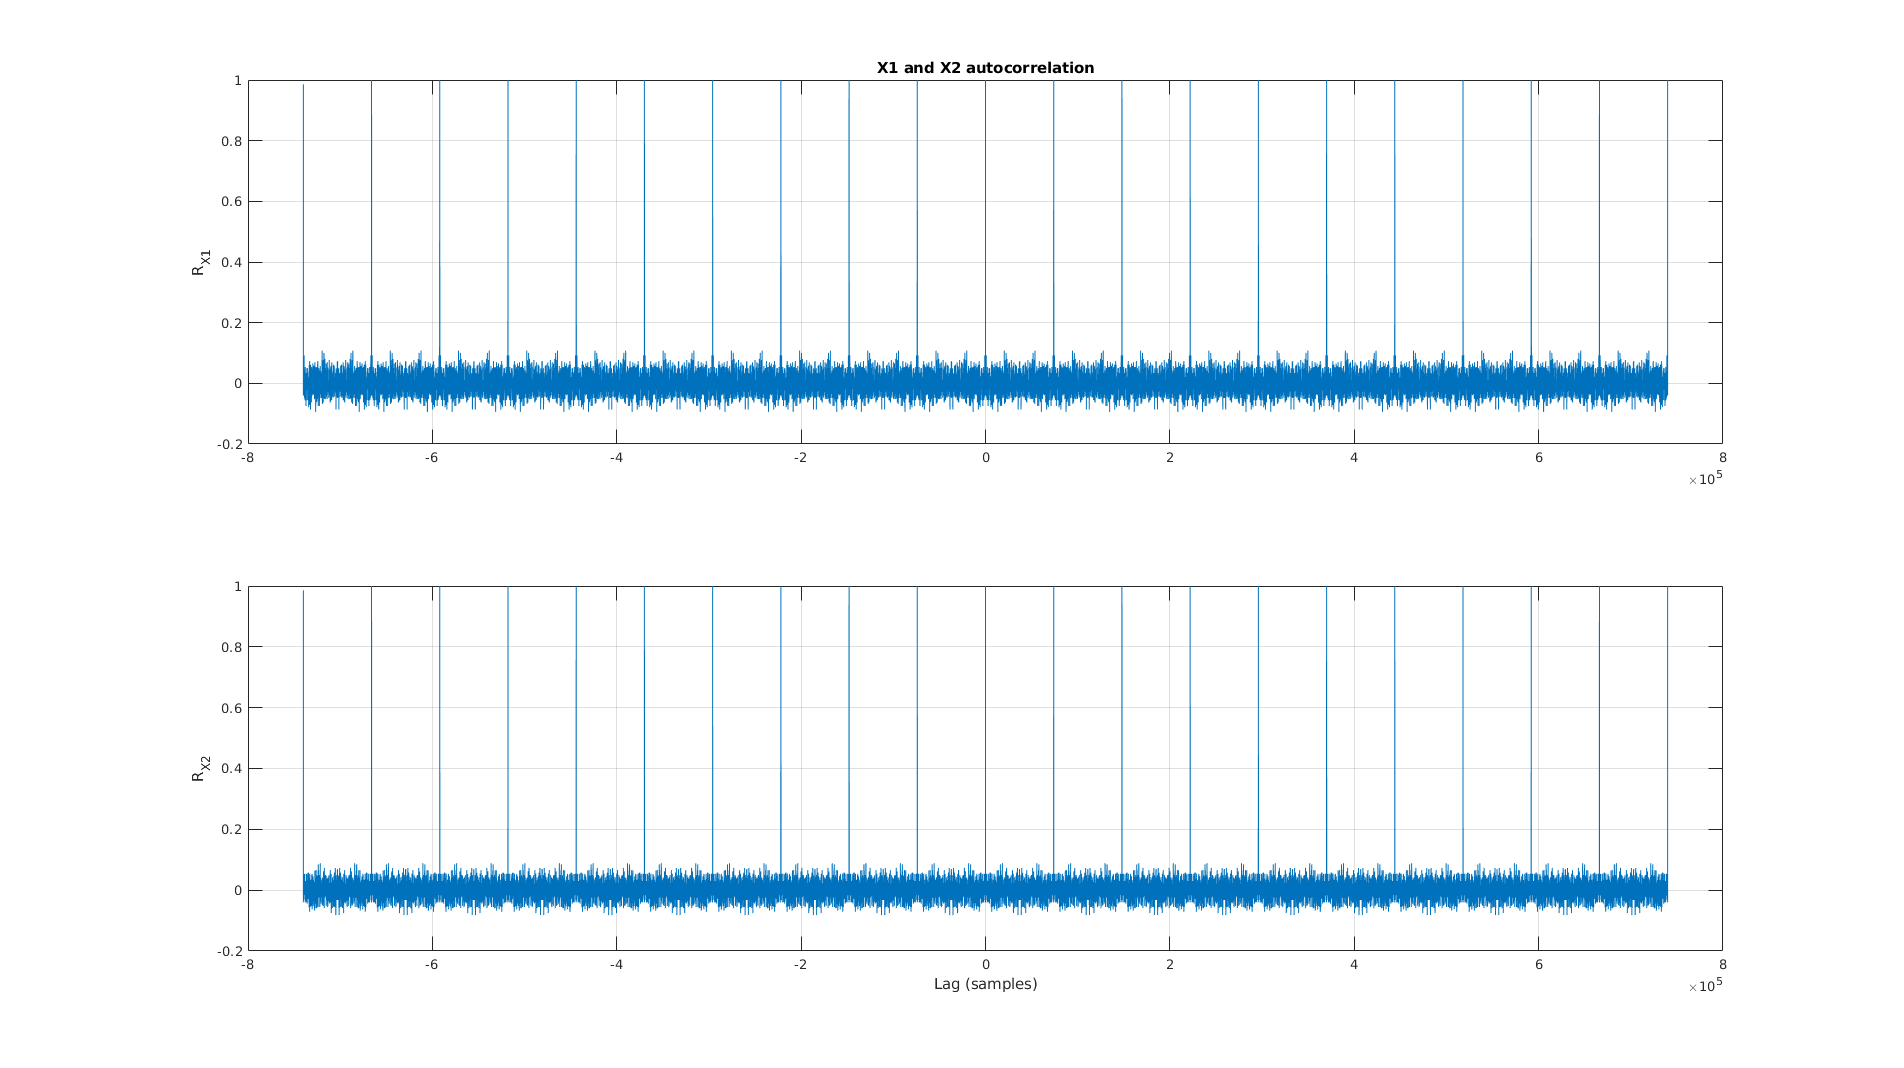
\includegraphics[width=0.9\textwidth]{figs/ex8_autocorr_pi.png}
	\caption{Autocorrelation of X1 and X2 for the 'pi' case.}
	\label{fig:ex8_autocorr_pi}
\end{figure}

\begin{figure}[H]
	\centering
	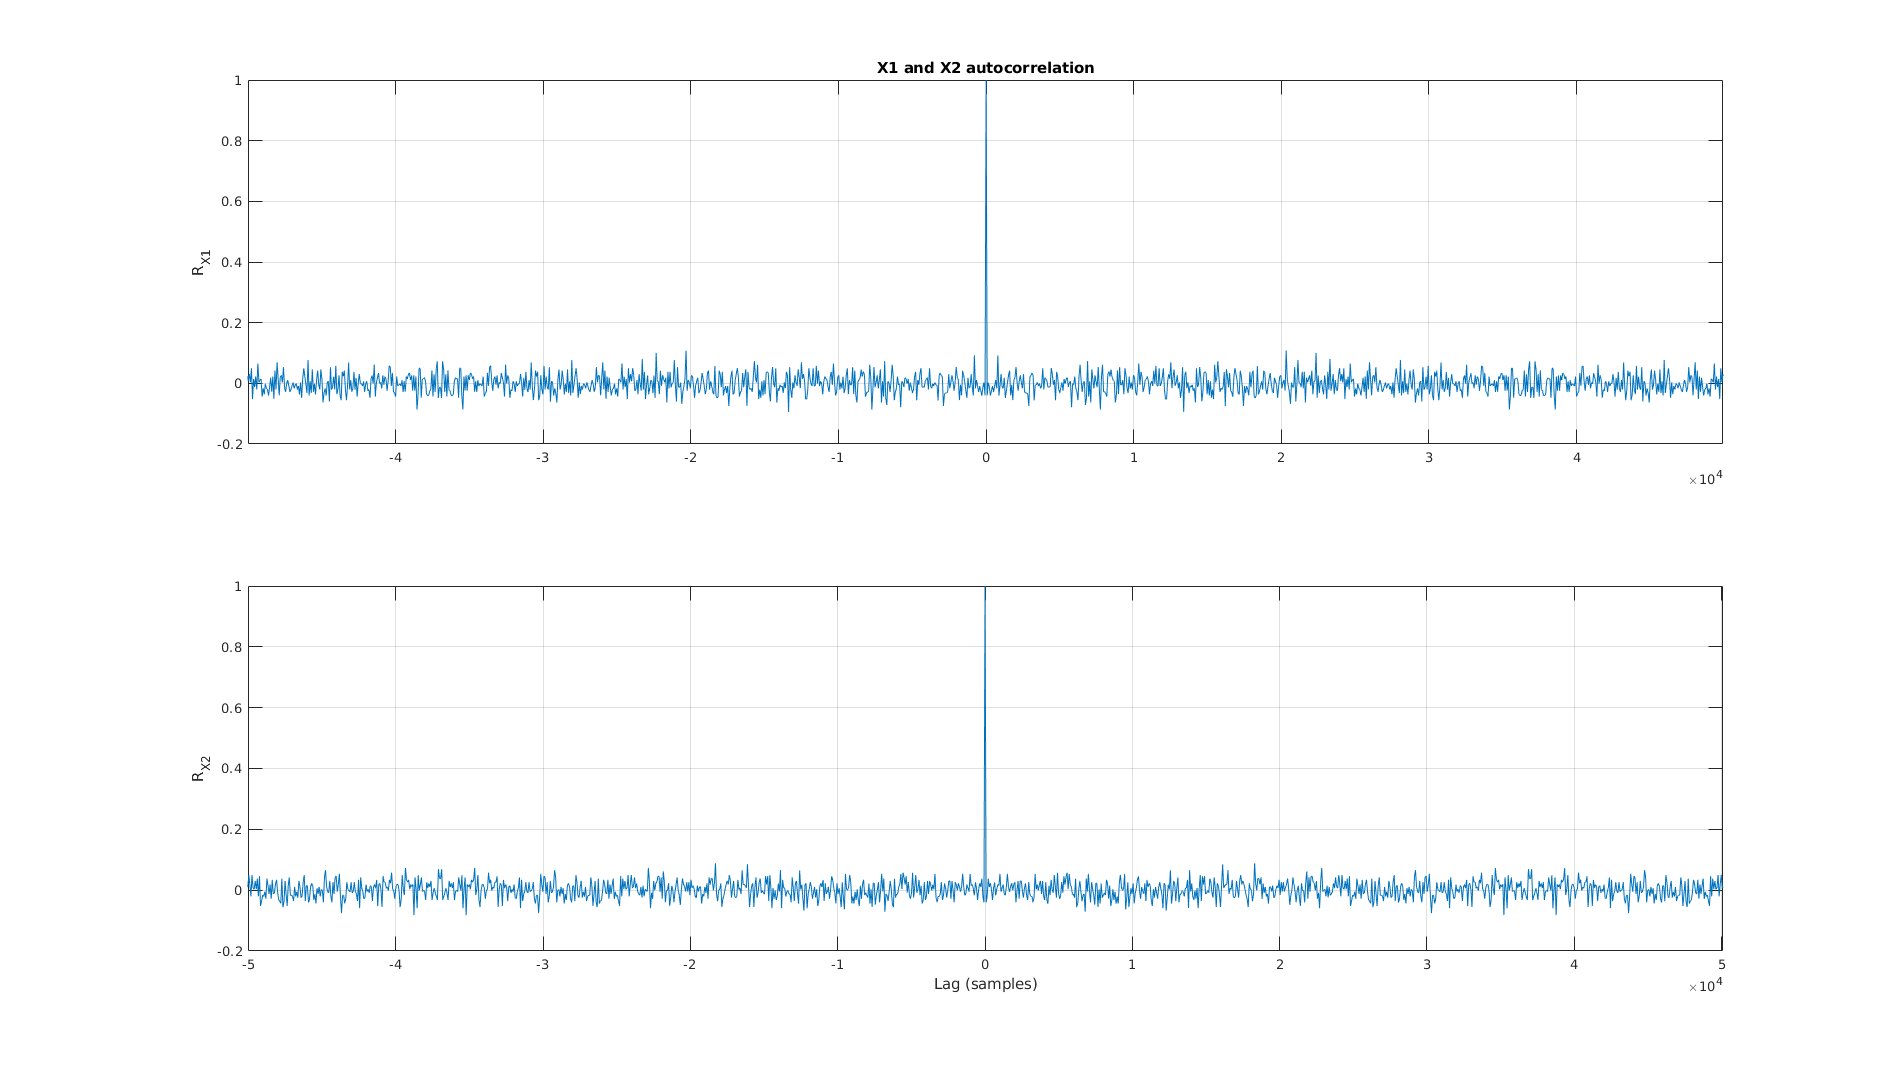
\includegraphics[width=0.9\textwidth]{figs/ex8_autocorr_zoomed_pi.png}
	\caption{Zoomed autocorrelation of X1 and X2 for the 'pi' case.}
	\label{fig:ex8_autocorr_zoomed_pi}
\end{figure}

The ratio of the maximum of $R_X(\tau)$ to the maximum of $R_{X1,X2}(\tau)$ is
10.12 for the case where we work with 'pi' method.

\begin{figure}[H]
	\centering
	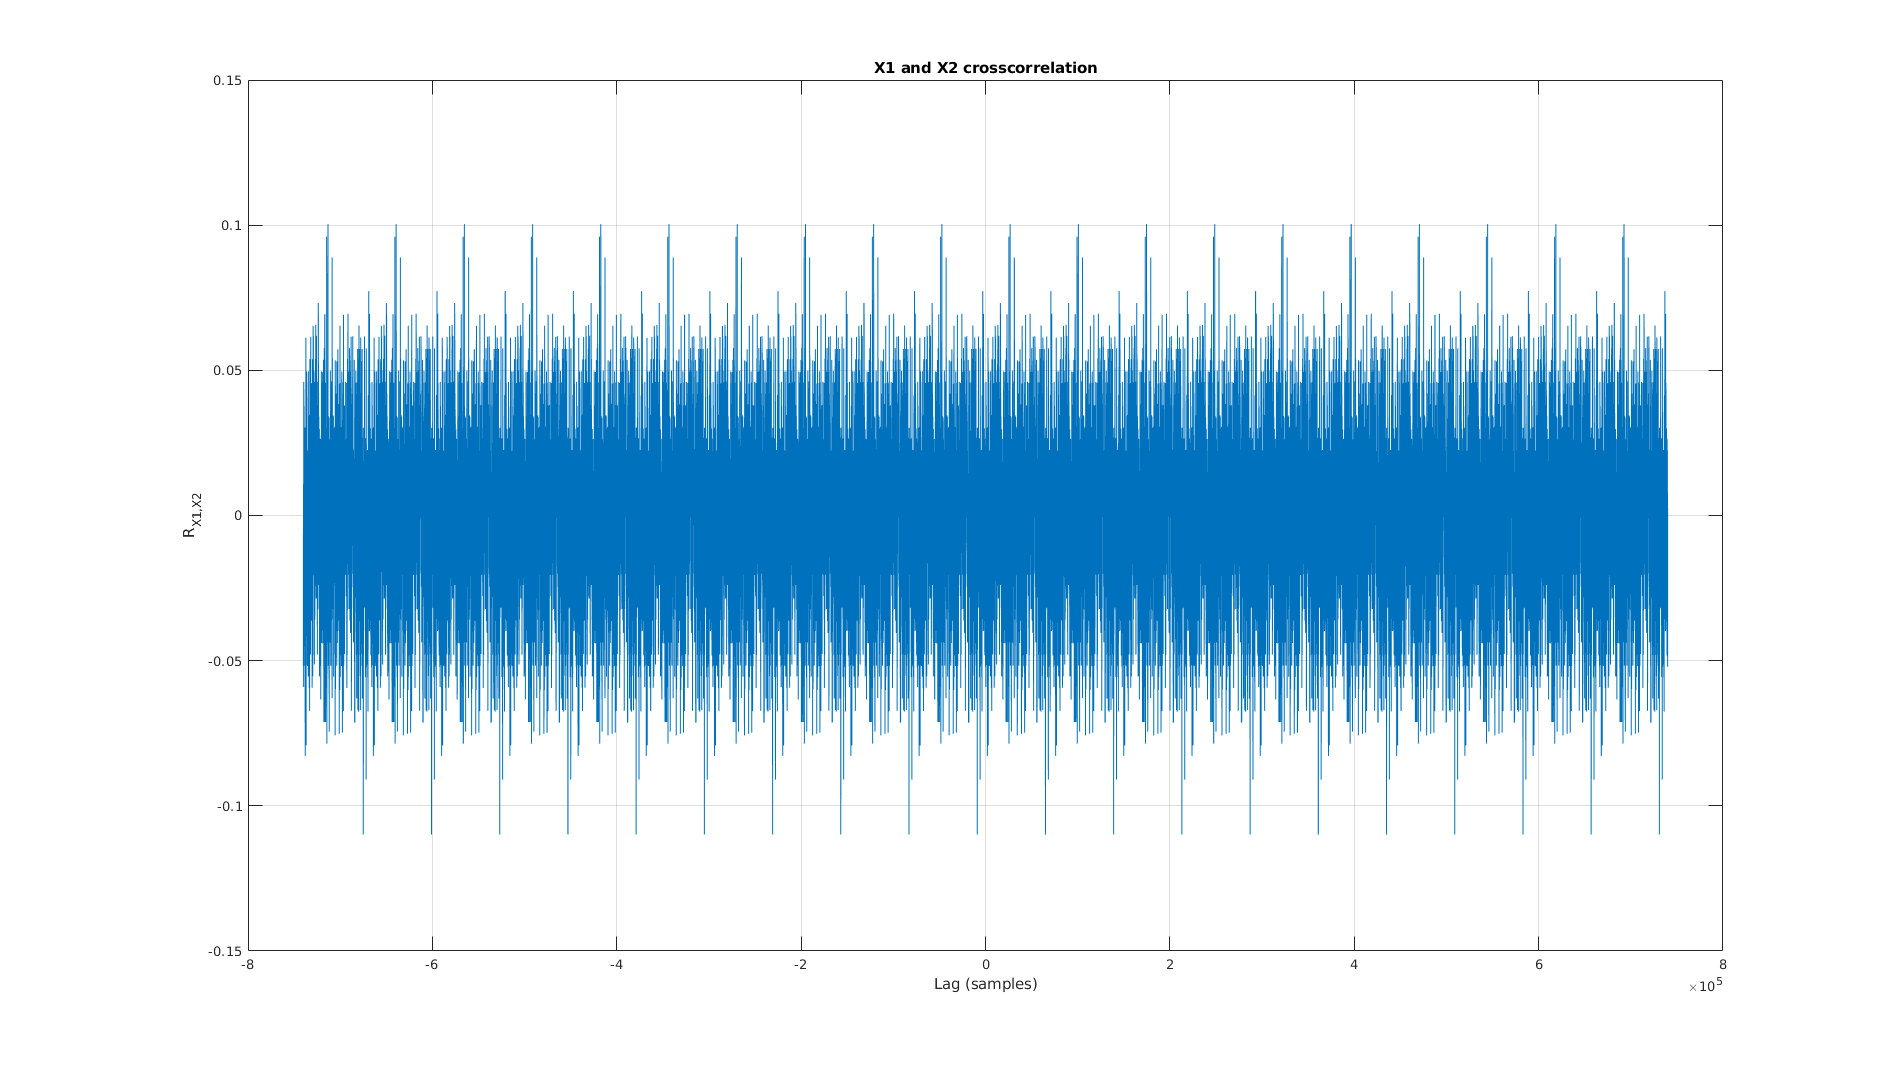
\includegraphics[width=0.9\textwidth]{figs/ex8_crosscorr_mseq.png}
	\caption{Crosscorrelation of X1 and X2 for the 'mseq' case.}
	\label{fig:ex8_crosscorr_mseq}
\end{figure}

\begin{figure}[H]
	\centering
	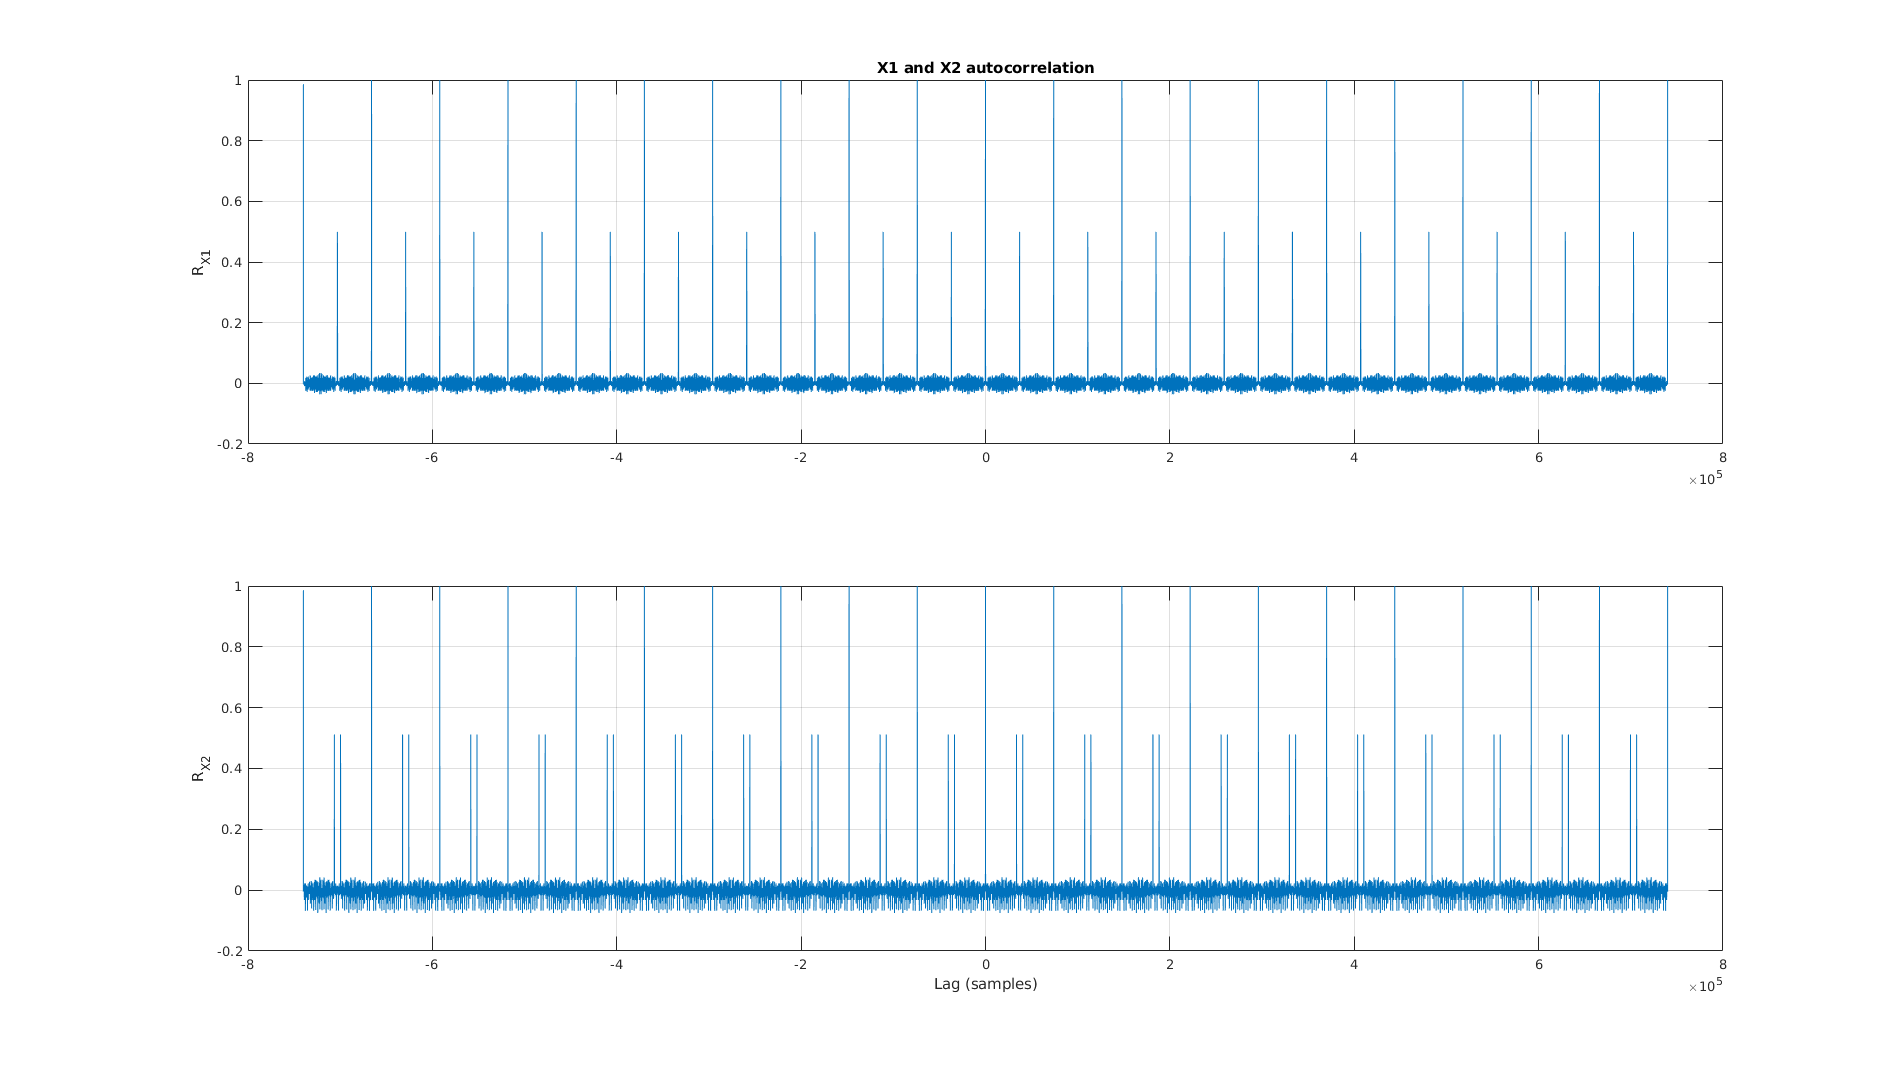
\includegraphics[width=0.9\textwidth]{figs/ex8_autocorr_mseq.png}
	\caption{Autocorrelation of X1 and X2 for the 'mseq' case.}
	\label{fig:ex8_autocorr_pi}
\end{figure}

\begin{figure}[H]
	\centering
	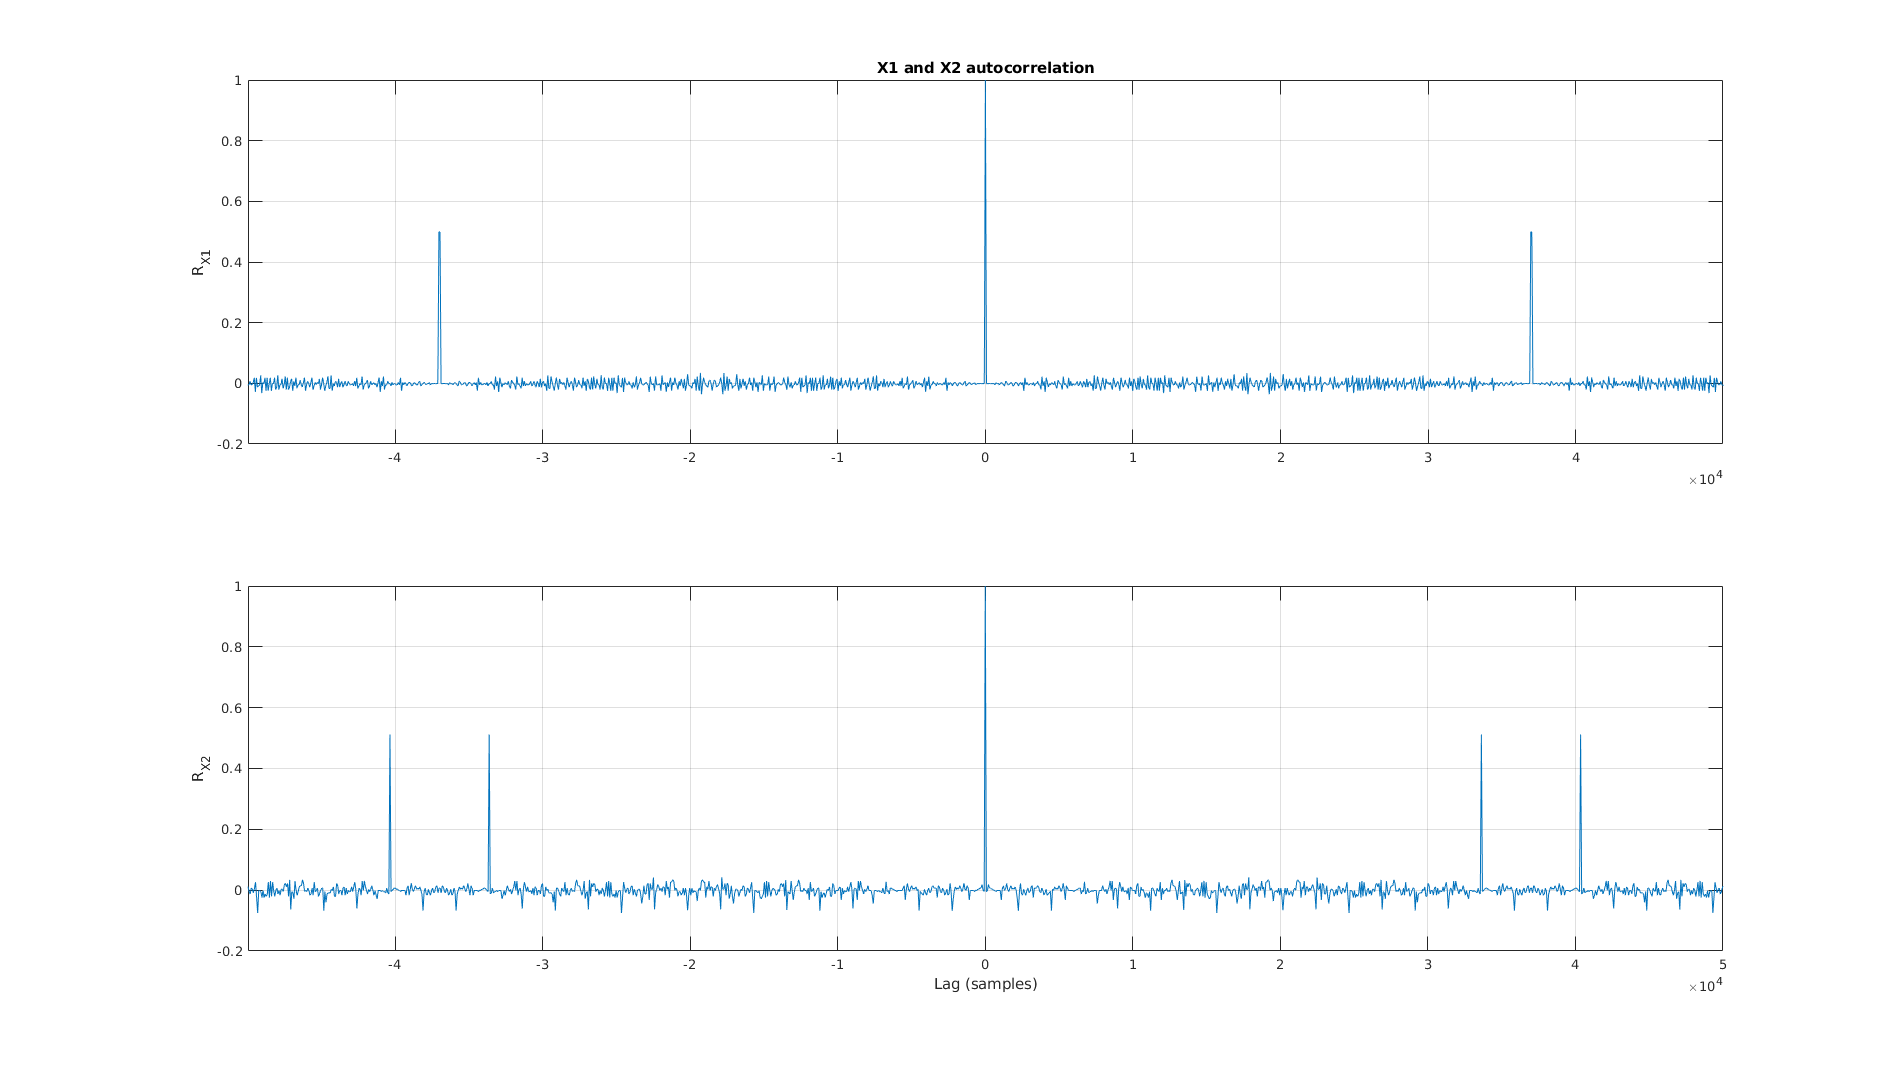
\includegraphics[width=0.9\textwidth]{figs/ex8_autocorr_zoomed_mseq.png}
	\caption{Zoomed autocorrelation of X1 and X2 for the 'mseq' case.}
	\label{fig:ex8_autocorr_zoomed_mseq}
\end{figure}

The ratio of the maximum of $R_X(\tau)$ to the maximum of $R_{X1,X2}(\tau)$ is
9.9659 for the case where we work with 'mseq' method.

Analyzing the graphs it's hard to conclude which method provides the best
cross-correlation properties. They all look very similar, showing values
concentrated below arround +-0.05 and spikes upto +-0.1. The ideal behavior we
are looking for is a cross-correlation equal to zero. Which would indicate that
no two signal could be confused because they are perfectly orthogonal.

The analysis of the autocorrelation is a little different. The 'rand' and 'pi'
methods look very similar. But the 'mseq' method is quite different. It has a
much lower floor, which it's closer to the ideal case we are looking for: the
Dirac delta. However, it presents smaller spikes to the sides. This could be
pretty bad because one could confuse this smaller peaks with the main peak and
consequently get an inaccurate range measurement due to pourly "locking" to the
local replica of the code. In addition to the aforementioned, the calculated
ratios show that the 'rand' method provides the greater relationship between
max autocorrelation and max cross-correlation, which is a desired property since
it means that there are more chances of correctly identifing and 'locking' to
the desired satellite's code. This result surprised me since I was expecting the
mseq to have the best properties.

% \section{Problem 9}

\section{Instruction}

Download the Cornell Scintillation Simulation Toolkit from
http://radionavlab.ae.utexas.edu/datastore/websiteFiles/scintSim.zip.
Read the instructions in UserGuide.pdf for generating synthetic scintillation.
Experiment with the graphical user interface by typing guiscint at the Matlab
prompt. You’ll be able to generate a time history of the complex channel
response function $z(t)$ by setting the parameters S4 and $\tau_0$ and pressing
‘Simulate’. The quantity Te above the bar chart is the mean time between
differentially-detected bit errors, which serves as a proxy for the mean time
between cycle slips. Notice how Te changes as you experiment with different
values of S4, $\tau_0$, and C/N0. Write your own Matlab function to calculate
the S4 index and the decorrelation time $\tau_0$ corresponding to a given
scintillation time history produced by the scintillation simulator and stored in
scintDat.mat. Test your function to see how well your calculated S4 and $\tau_0$
values match the values that were used as parameters in generating the data.

\subsection{Solution}


\begin{lstlisting}
function [S4,tau0] = computeS4AndTau0(zkhist,tkhist)
% computeS4AndTau0 : Compute the scintillation index S4 and the decorrelation
%                    time tau0 corresponding to the input complex channel
%                    response function time history zkhist.
%
% INPUTS
%
% zkhist ----- Nt-by-1 vector containing the normalized complex scintillation
%              time history in the form of averages over Ts with sampling
%              interval Ts. zkhist(kp1) is the average over tk to tkp1.
%
% tkhist ----- Nt-by-1 vector of time points corresponding to zkhist.
%
%
% OUTPUTS
%
% S4 --------- Intensity scintillation index of the scintillation time history
%              in zkhist, equal to the mean-normalized standard deviation of
%              the intensity abs(zkhist).^2.
%
% tau0 ------- The decorrelation time of the scintillation time history in
%              zkhist, in seconds.
%
%
%+------------------------------------------------------------------------------+
% References:
%
%
%+==============================================================================+
alpha = abs(zkhist);
I = alpha.^2;
S4_squared = (mean(I.^2) - mean(I)^2) / mean(I)^2;
S4 = sqrt(S4_squared);

z_bar = mean(zkhist);
xi = zkhist - z_bar;
[R,lags] = xcorr(xi,'normalized'); 
idx = find(abs(R(find(lags==0):end)) < R(find(lags==0))*exp(-1), 1);
tau0 = tkhist(idx);
\end{lstlisting}


%\bibliographystyle{ieeetr}
%\bibliography{./pangea}  
\end{document}
